\documentclass[12pt,a4paper]{scrartcl}
\usepackage[utf8]{inputenc}
%\usepackage[latin1]{inputenc} %  Alternativ unter Windows
\usepackage[T1]{fontenc}
\usepackage[paper=a4paper,
	left=25mm,
	right=25mm,
	top=25mm,
	bottom=20mm]{geometry}
\usepackage[nottoc]{tocbibind}
\usepackage[ngerman]{babel}
\usepackage[pdftex]{graphicx}
\usepackage{latexsym}
\usepackage{amsmath,amssymb,amsthm,amsfonts}
\usepackage{mathtools}
\usepackage{physics}
\usepackage{enumitem}
\usepackage[utf8]{inputenc}
\usepackage{float}
\usepackage{subfigure}
\newcommand{\R}{\mathbb{R}}

\DeclareMathOperator{\dive}{div}
\newtheorem{Satz}{Satz}[section]\newtheorem{Definition}[Satz]{Definition} 
\newtheorem{Lemma}{Lemma}		                 
\newtheorem{Korollar}[Satz]{Korollar}
\newtheorem{Proposition}[Satz]{Proposition}                  
\newtheorem{examples}[Satz]{Beispiel}
\let\oldexamples\examples
\renewcommand{\examples}{\oldexamples\normalfont}
\newtheorem*{notation}{Notation}
\let\oldnotation\notation
\renewcommand{\notation}{\oldnotation\normalfont}
\newtheorem*{remark}{Bemerkung}
\let\oldremark\remark
\renewcommand{\remark}{\oldremark\normalfont}                  


\usepackage[german=quotes]{csquotes}
\usepackage{xcolor}
\newcommand*\diff{\mathop{}\!\mathrm{d}}
\DeclareMathOperator{\conv}{conv}
\DeclareMathOperator{\spann}{span}
\DeclareMathOperator{\Jacobi}{D}
\DeclareMathOperator{\diam}{diam}
\definecolor{Mygreen}{RGB}{0,128,0}
\newcommand{\defi}[1]{\textcolor{Mygreen}{#1}}
\renewcommand{\phi}{\varphi}
\renewcommand{\epsilon}{\varepsilon}
                              
\numberwithin{equation}{section} 

% Praktikumsbericht nummer setzen
\newcommand{\BerichtNR}{1}

\begin{document}
\begin{titlepage}
	
\includegraphics[scale=0.5]{kit-logo.jpg} 
	\begin{center} 
		\LARGE 
		\vspace*{2cm}
		\LARGE Praktikumsbericht \BerichtNR
		\vspace*{1.0cm}
		\hrule
		\vspace*{0.2cm}
		{\vspace{0.2cm} \huge Einführung in das Wissenschaftliche Rechnen}\vspace{0.5cm}
		\hrule
		\vspace*{2.5cm}
		\Large Stefan Karch \\
		Florian Döttling \\
		Tim Buchholz  \\
		\vspace*{1cm}
		20.05.2019 \\
		\vspace*{1.5cm}
		\vspace*{4.0cm}
		\Large Betreuung: Prof. Dr. Christian Wieners, Niklas Baumgarten \\[0.5cm]
		\Large Fakultät für Mathematik \\
		\Large Karlsruher Institut für Technologie
	\end{center}
\end{titlepage}

%\tableofcontents
%\newpage 
%\pagestyle{headings}

\section{Problemstellung}

\begin{enumerate}[label=(\roman*)]
\item Problemdarstellung: Woraus leitet sich das Modellproblem der Regenwasserversickerung aus Aufgabe 4 ab?
\item Mathematisches Modell: Welcher Lösungsansatz wird gewählt?
\item Numerische Methoden: Wie sind die numerischen Methoden konstruiert und konfiguriert?
\item Beschreibung  Funktionsweisen  von M++:  Gebietsaufteilung/Lastverteilung,  Geometriedefinitionen, Gitterverfeinerung und Zusammenhang zum Level.
\item Ergebnisse aus den Aufgaben: Visualisieren, interpretieren und arbeiten Sie Ihre Erkenntnisse aus Aufgabe 4 aus.
\item Visualisieren, interpretieren und arbeiten Sie Ihre Erkenntnisse aus Aufgabe 6 aus.
\end{enumerate}

\section{Ergebnisse}

\begin{enumerate}[label=(\roman*)]
\item  $ \Omega \subseteq \R^3 $  beschreibe eine poröse Bodenschicht. Von oben sickert Regenwasser langsam ins Grundwasser. Das Ziel ist nun, die transportierte Wassermenge und deren Verteilung zu bestimmen.
\newline Durch das Darcy-Gesetz $ q= -\kappa(\nabla p - G)$ wird der Fluss eines Fluids beschrieben, bei dem 
\begin{align*}& p:\Omega \rightarrow \R &&\text{den hydrostatische Druck,}\\
&  \kappa : \Omega \rightarrow (\R_{sym})^{3\times3}  &&\text{den Permeabilitätstensor}\\
& G = (0,0,\rho_0 g_0)^T &&\text{die Gravitation}
\end{align*} beschreiben. Durch $u(x):=-p(x)+\rho_0 g_0 x_3$ vereinfacht sich das Darcy-Gesetz zu $q=\kappa\nabla u$.
\newline Sei $\partial \Omega = \Gamma_N \cup \Gamma_D$. Durch die Vorgabe von Funktionen auf dem Rand von $\Omega$ mit
\begin{align*}&u_D: \Gamma_D \rightarrow \R &&\text{(Dirichlet-Werte)}\\
& g_N: \Gamma_N \rightarrow \R &&\text{(Neumann-Werte)}
\end{align*} ergibt sich schließlich die Randwertaufgabe: Bestimme $u:\bar{\Omega} \rightarrow \R$ mit
\[(1)\begin{cases}
\dive \kappa \nabla u = 0 &\text{in $\Omega$}\\
u = u_D  &\text{auf $\Gamma_D$}\\
\kappa \nabla u \cdot \nu = g_N &\text{auf $\Gamma_N$}
\end{cases}
\]
Dabei bezeichnen wir den äußeren Normalenvektor mit $\nu$.
\newline Zur Vereinfachung des Problems (1) nehmen wir nun einen Querschnitt an der Stelle $x_2 = 0$, um das Problem auf einer zweidimensionalen Ebene zu betrachten. Diese Vereinfachung ist zulässig unter der Annahme, dass der Boden in der $x_2$-Richtung homogen ist. 
\newline Im Praktikum betrachten wir nun das folgende Problem:
\[(2)\begin{cases}
- \Delta u = 0 &,(x,y) \in \Omega = (0,1)^2\\
u(x,y) =0   &,y=0 \ \ \text{(Grundwasserspiegel)}\\
\nabla u(x,y) \cdot \nu = -1 &,y=1 \ \ \text{(Einflussströmung)}\\
\nabla u(x,y) \cdot \nu = 0 &,x\in \{0,1\}  \ \ \text{(Neumann-RB)}
\end{cases}
\]

\item Wir suchen eine Lösung der Randwertaufgabe (2).

Dazu führen wir wie in der Vorlesung einen schwachen Lösungsbegriff für obige Differentialgleichung ein: 

\fbox{\parbox{\linewidth}{
\begin{Lemma}
$\newline$
\begin{itemize} 
\item[a)] Sei $ \dive q = 0$ in $\Omega$. Dann gilt für alle Testfunktionen $\Phi : \Omega \rightarrow \R$  
\begin{align*}
\int_{\Omega}{q \nabla \Phi \diff x} = \int_{\partial \Omega}{\Phi q \cdot \nu \diff a}
\end{align*}
\item[b)] Sei $\int_{\Omega}{q \nabla \Phi \diff x} = \int_{\partial \Omega}{g \Phi \diff a}$ für alle Testfunktionen $\Phi : \Omega \rightarrow \R$. Dann gilt 
\begin{align*}
\dive q = 0 \text{ in } \Omega  \text{ und } q \cdot \nu = g \text{ auf } \partial \Omega
\end{align*}
\end{itemize}
\end{Lemma}
}}
$\newline$
Konkret suchen wir also einen Fluss q, der der Bedingung aus b) genügt, denn gilt  
\begin{align*}
\int_{\Omega}{q \nabla \Phi dx} = \int_{\partial \Omega}{g \Phi da} = 0 \quad \forall \Phi : \Omega \rightarrow \R \text{ mit } \Phi = 0 \text{ auf }\partial\Omega  
\end{align*}
dann gilt: 
\begin{align*}
\dive q = 0 \text{ in } \Omega \text{ (fast überall im Sinne von } L_2 \text{)}
\end{align*}
Insbesondere ist dann:
\begin{align*}
\int_{\partial \Omega}{\Phi q \nu da} = \int_{\partial \Omega}{\Phi g da} \Rightarrow q \cdot \nu = g \text{ auf } \partial \Omega
\end{align*} 
\newline
Konkret kommen wir so also von 


\[
\begin{cases}
\dive q = 0 \text{ , }  q = - \kappa  \nabla u  \text{ in }  \Omega \text{ }\\
-q \cdot \nu = g_N  \text{ auf } \Gamma_N \\
 u = u_D \text{ auf } \Gamma_D
\end{cases}
\]

zur \defi{schwachen Form} unseres Problems:
\begin{align*}
\int_{\Omega}{ \kappa \nabla u \cdot \nabla \Phi dx} = \int_{ \Gamma_N }{g_n \Phi da} \text{  } \; \; \forall \Phi \text{ mit } \Phi = 0 \text{ auf } \Gamma_D
\end{align*}

\item
Aus der schwachen Form der Problemstellung in Ergebnis (ii) leitet sich die diskrete Formulierung her. Dazu wurde der unendlich-dimensionale Raum der Testfunktionen $V$ auf den endlich-dimensionalen Testraum $V_h$ eingeschränkt. Und auch die Lösung wird im endlich-dimensionalen $V_h$ gesucht. Somit erhält man das Problem
\begin{align*}
&\text{Bestimme } u_h \in V_h \text{ mit }\\
&(\star)\begin{cases}
	\int_{\Omega} \kappa \nabla u_h \cdot \nabla \Phi_h \diff x = \int_{\Gamma_N} g_N  \Phi_h \diff a \text{ (für alle } \Phi_h \in V_h \text{ mit } \Phi_h = 0 \text{ auf } \Gamma_D) \\
	u_h \approx u_D \text{ auf } \Gamma_D
\end{cases}
\end{align*}
Was $ V_h $ ist, ist noch fraglich und wird im Folgenden hergeleitet.
\begin{description}
	\item [zu $\Omega$:]
	Wir betrachten nur den Spezialfall: $\Omega \subseteq \R^2$ ein Polygongebiet. 
	
	Es sei $\mathcal{K}$ eine Zerlegung von $\Omega$ bestehend aus Dreiecken oder Vierecken.
	\begin{align*}
	\text{Also} \bigcup_{K \in \mathcal{K}} \overline{K} = \overline{\Omega} \text{ und } \overline{K} = \conv \mathcal{V}_K \text{, und}\\
	\mathcal{V}_K \coloneqq
	 \begin{cases}
	\{z_{K,0}, z_{K,1}, z_{K,2}\} \subseteq \R^2, &\text{für Dreiecke} \\
	\{z_{K,0}, z_{K,1}, z_{K,2}, z_{K,3}\} \subseteq \R^2, &\text{für Vierecke}
	\end{cases}
	\end{align*}
	
	Ein $ K \in \mathcal{K} $ heißt \defi{Zelle}, ein $ z \in \mathcal{V}_h $ heißt \defi{Knoten} und die Menge aller Knoten sei $\mathcal{V}_\mathcal{K} \coloneqq \bigcup_{K \in \mathcal{K}} \mathcal{V}_K$
	
	Weiterhin fordern wir, dass die Zerlegung $\mathcal{K}$ zulässig ist, d.h. der Schnitt zwei verschiedener Zellen ist leer, eine Ecke oder eine Kante.
	
	\item[zu $V_K$:] 
	Die numerische Lösung $u_h$ wird durch die Werte $ u_h(z) $ an allen Knoten $z \in \mathcal{V}_\mathcal{K}$ bestimmt. $ u_h $ wird linear auf jedem $K \in \mathcal{K}$ interpoliert und auf $ \Omega $ zusammengesetzt.
	
	Für die Interpolation auf einem $ K \in \mathcal{K} $ betrachten wir den Testraum, welcher von \enquote{Hütchenfunktionen} aufgespannt wird. Für alle $ \{z_{K,0},\dots, z_{K,N_K} \} = \mathcal{V}_K $ ist die Hütchenfunktionen $ \lambda_{K,i}\colon K \to \R \ $ gegeben durch
		\[
			\lambda_{K,i}(z_{K,j}) = \delta_{i,j}
			\text{ und dazwischen linear interpoliert.}
		\] 
		Um die Hütchenfunktionen $ \{\lambda_{K,i}\} $ auf $ K $ zu berechnen, verwenden wir die Hütchenfunktionen $ \{\hat{\lambda_i}\} $ auf der \defi{Referenzzelle} (Referenzdreieck oder Referenzviereck) $ \hat{K} $. Mit einer Koordinatentransformation von $ \hat{K} $ nach $ K $
		\begin{align*}
			\phi_K\colon \hat{K} \to \overline{K}, \phi_K(\xi) \mapsto z_{K,0} + B_K(\xi) \quad \text{mit} \quad B_K(\xi) = \Jacobi\phi_K(\xi)
		\end{align*}
		erhalten wir die Hütchenfunktionen auf $ K $ durch
		\begin{align*}
			\lambda_{K,i} = \hat{\lambda}_i \circ \phi_K^{-1}.
		\end{align*}
		Weiter sei
		\begin{align*}
			V_K \coloneqq \spann\{\lambda_{K,i}: i=0,1,\dots,N_K\}
		\end{align*}
		der \enquote{Ansatzraum} (oder \enquote{Testraum}) auf $ K $. 
	
\item[zu $ V_h $:] Zu einer gegebenen Zerlegung $\mathcal{K}$ mit \defi{maximaler Kantenlänge} $ h \coloneqq \max_{K \in \mathcal{K}} \diam(K) $ werden die \defi{Finite-Elemente-Ansatzräume} 
	\begin{align*}
		V_h \coloneqq \{ \Phi_h \in C(\overline{\Omega}): \Phi_h|_K \in V_K \ (K \in \mathcal{K})\}
	\end{align*}
	und
	\begin{align*}
		V_h(u_D) \coloneqq \{ \Phi_h \in V_h: \Phi_h(z)=u_D(z) \ (z \in \mathcal{V}_\mathcal{K} \cap \Gamma_D) \}
	\end{align*}
	definiert.
	
\end{description}

Somit kann die diskrete Problemstellung $ (\star) $ nun  formuliert werden:
	\begin{align*}
		&\text{Bestimme } u_h \in V_h(u_D) \text{ mit }\\
		&\begin{cases}
		\sum_{K \in \mathcal{K}} \int_{K} \kappa \nabla u_h \cdot \nabla \Phi_h \diff x = \int_{\Gamma_N} g_N  \Phi_h \diff a \text{ für alle } \Phi_h \in V_h(0)
		\end{cases}
	\end{align*}

Als nächsten Schritt wollen wir unser diskretes Problem in ein lineares Gleichungssystem umformulieren. 
	Mit der Basis $ \{\lambda_1, \dots , \lambda_N\} $ (\defi{Knotenbasis}/\emph{globale Hütchenfunktionen})von $V_h$ mit
	\begin{align*}
		&\forall z_k \in \mathcal{V}_\mathcal{K} \ \lambda_i(z_k) = 
		\begin{cases}
			1, &n=k\\
			0, &n\neq k
		\end{cases}
		\ &&(\text{dazwischen interpoliert})\\
	\text{und} \\
		&\mathcal{I} \coloneqq \{ 1, \dots , N \}  &&\text{\defi{Indexmenge der Knoten}} \\
		&\mathcal{I}_D \coloneqq \{ h \in \mathcal{I} : z_h \in \Gamma_D \}  &&\text{\defi{Indexmenge der Knoten, auf dem Dirichletrand }}
	\end{align*}
	erhalten wir die Problemstellung:
	\begin{align*}
		&\text{Bestimme } \underline{u} \in \R^N \text{ mit }\\
		&\begin{cases}
			\sum_{n = 1}^N \underline{u}_n \lambda_n = u_h  \\
			\sum_{n=1}^{N} \underline{u}_n \sum_{k \in \mathcal{K}} \int_{K} \kappa \nabla \lambda_n \cdot \nabla \lambda_k \diff x = \int_{\Gamma_N} g_N \lambda_k \diff a (k \in \mathcal{I}\setminus\mathcal{I}_D).
		\end{cases}
	\end{align*}
	Die erste Forderung an $ \underline{u} $ bedeutet, dass $\underline{u} $ der Koordinatenvektor von $ u_h~\in~V_h(u_D) $ in der Knotenbasis  $ \{ \lambda_i \}_{i = 1}^N $ ist.
	
	Ein LGS erhalten wir durch die Steifigkeitsmatrix und den Lastvektor. 
	
	Sei $\underline{A} \in \R^{N \times N} $ die \defi{Steifigkeitsmatrix} mit 
	\begin{align*}		
		\underline{A}[k,n] \coloneqq
		\begin{cases}
			\sum_{K \in \mathcal{K}} \int_K \kappa \nabla \lambda_n \cdot \nabla \lambda_k \diff x, & k \notin \mathcal{I}_D \text{ oder } n \notin \mathcal{I}_D \\
			1, & n,k \in \mathcal{I}_D \text{ und } n = k\\
			0, & n,k \in \mathcal{I}_D \text{ und } n \neq k 
		\end{cases}
	\end{align*}
	und $\underline{b} \in \R^N $ der \defi{Lastenvektor} mit
	\begin{align*}
		\underline{b}[k] \coloneqq
		\begin{cases}
			\int_{\Gamma_N} g_N \lambda_k \diff a, & k \notin \mathcal{I}_D \\
			u_D(z_k), & k \in \mathcal{I}_D.
		\end{cases}
	\end{align*}
	Dann lautet das zu lösende Problem:
	\begin{align*}
			\text{Bestimme } \underline{u} \in \R^N \text{ mit } \underline{A}\, \underline{u} = \underline{b}.			
	\end{align*}
	Nach Konstruktion von $\underline{A}$ und $ \underline{b} $ gilt $\underline{u}_k = u_D(z_k) \ (k\in \mathcal{I}_D)$.
	
	Diese Problem ist wohldefiniert, bzw. $ \underline{A} $ ist regulär, falls $ \kappa $ uniform symmetrisch positiv definit ist und $ \Gamma_D \cap \mathcal{V}_\mathcal{K} \neq \emptyset$ (Es gibt mindestens einen Knoten auf dem Dirichletrand).
	
	\defi{Assemblieren} bezeichnet den Vorgang des Bestimmens von $ \underline{A} $ und $ \underline{b}$. Dabei wird in jeder Zelle $ K \in \mathcal{K} $ mit den Einschränkungen auf $ K $ von der Knotenbasis $ \{ \lambda_{K,i} \}_{i=1}^N $ gerechnet. Die Einschränkung von $ \lambda_n $ heißen $ \lambda_{K,n} $.
	\begin{align*}
		\underline{A}[n,k] = \sum_{K \in \mathcal{K}} \int_{K} \kappa \nabla \lambda_{K,k} \cdot \nabla \lambda_{K,n} \diff x \ (k \notin \mathcal{I}_D \text{ oder } n \notin \mathcal{I}_D)
	\end{align*}
	Auf den einzelnen Zellen wird das Integral mithilfe der Transformation auf die Referenzzelle und Quadraturverfahren bestimmt.
	
		
	Für eine Matrix $ M \in \R^{N \times N} $ heißt $ \mathcal{I} \coloneqq \{1 , \dots , N\} $ \defi{Indexmenge} und
	$ G_M \coloneqq  \{(n,k) \in \mathcal{I} \times \mathcal{I} : A[n,k] \neq 0 \} $ \defi{Matrixgraph}. M heißt \defi{dünn besetzt} , wenn $ |G_A| = \mathcal{O}(N) $. Sonst heißt M \defi{voll besetzt}.
	
	Viele der Einträge in $ \underline{A} $ sind 0, da viele Funktionen aus der Knotenbasis $ \{ \lambda_{K,i} \}_{i = 1}^N $ paarweise disjunkte Träger haben. Somit handelt es sich bei $ \underline{A} $ in der Regel um eine dünn besetzte Matrix.
	

\item Zur Gebietsaufteilung/Lastverteilung: \newline
Über das in der Vorlesung eingeführte Schurkomplement haben wir die Möglichkeit gegeben, das in (iii) hergeleitete LGS parallel zu lösen. Dabei ist wichtig, dass die Interfaces, also die Abhängigkeiten zwischen den einzelnen Blöcken (Gebiet / Teil-LGS welches ein Prozessor berechnet) möglichst klein zu halten. \newline
Um dies zu gewährleisten, haben wir in der Vorlesung verschiedene Partitionierungsalgorithmen kennengelernt. 
Unter anderem 'RCB', 'RIB' oder 'Space Filling Curves'.
\newline
\par
Die Geometriedefinition in M++ erfolgt über Geofiles. Im Folgenden gehen wir kurz anhand eines Beispieles auf ein solches ein: \newline

\begin{figure}[H]
	\centering
	\captionabove{Aufbau der Geofiles am Beispiel von 'UnitSquare.geo':}
		 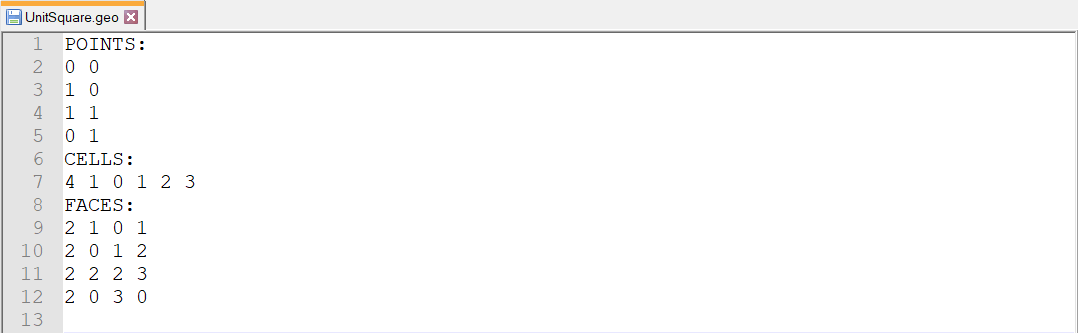
\includegraphics[width=\textwidth]{../Geobeispiel.png}
\end{figure}
Im ersten Block werden die Punkte in Form von zwei Koordinaten definiert. M++ skaliert diese intern auf das Einheitsquadrat. Wichtig ist die Reihenfolge der Punkte da wir später nur noch über den Index des Punktes auf den Punkt zugreifen. \newline
Im zweiten Block definieren wir die Zellen der Triangulierung innerhalb des Einheitsquadrates.
Der erste Eintrag steht für die Anzahl der Ecken. Der zweite Eintrag ist ein 'Flageintrag' und macht es möglich einzelne Zellen zu markieren. 
Die restlichen Einträge stehen für die Punkte im mathematisch positiven Sinn. 
Im dritten und letzten Block werden die Faces/Ränder definiert. Dabei steht der erste Eintrag für die Anzahl der Punkte (eigentlich machen hier aber nur Kanten Sinn, also 2 Punkte). Der zweite Eintrag steht für die Art des Randes. Hierbei steht 
\begin{enumerate}
\item 0 für einen Neumann-0-Rand (Neumann Rand mit $g_N \equiv 0$) 
\item 1 für einen Dirichlet-Rand
\item 2 für einen Neumann-Rand mit $g_N \not\equiv 0$
\end{enumerate}
Wiederum stehen die restlichen Einträge für die zugehörigen Punkte. \newline
\par
\begin{figure}[H]
	\centering
	\captionabove{Gitterverfeinerung am Beispiel von 'UnitSquare'}
	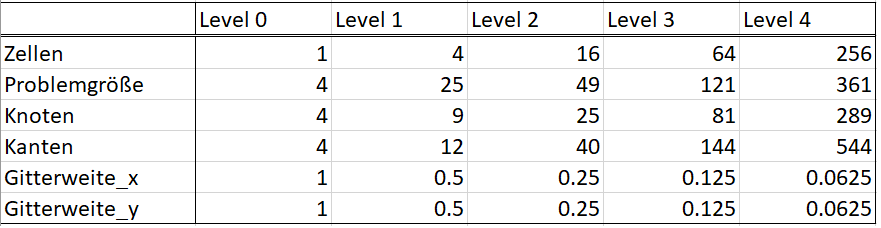
\includegraphics[width=\textwidth]{../Gitterverfeinerung.png} 
\end{figure}
Anhand der obigen Tabelle fällt es leicht, die Gitterverfeinerung nachzuvollziehen.
Auf Level 0 erhalten wir genau das Gitter, welches im Geofile definiert ist, also im Falle 'UnitSquare' genau eine Zelle mit 4 Ecken und 4 Kanten.
Anschließend wird mit jedem Level die Gitterweite sowohl in x- , als auch in y-Richtung halbiert. Daraus resultiert eine Vervierfachung der Zellen. \newline
Auf komplizierten Grundgittern fallen die einzelnen Werte natürlich anders aus, die Halbierung der Gitterweiten bzw. die Vervierfachung der Zellen sollte aber immer erkennbar sein. \newline
So ergeben sich beispielsweise auf 'Square500' auf Level 0 die Zellenanzahl 478 und die Gitterweiten (0.0625,0.0884) und auf Level 1 die Zellenanzahl 1912 und die Gitterweiten (0.03125,0.0442). 
\item Aufgabe 4
\newline

\begin{figure}[H]
	\centering
	\captionabove{Permeabilitäten der Probleme Simple und Discontinuous}
	\subfigure[Problem Simple]{
\includegraphics[width=0.49\textwidth]{../Problem_Simple2DMesh_UnitSquare8Triangelslevel_7/perm2.png}}	 
	\subfigure[Problem Discontinuous]{
\includegraphics[width=0.49\textwidth]{../Problem_DiscontinousMesh_UnitSquarelevel_8/perm2.png}}	
\end{figure}

%\begin{figure}[H]
%	\centering
%	\captionabove{Permeabilität bei Simple:}
%		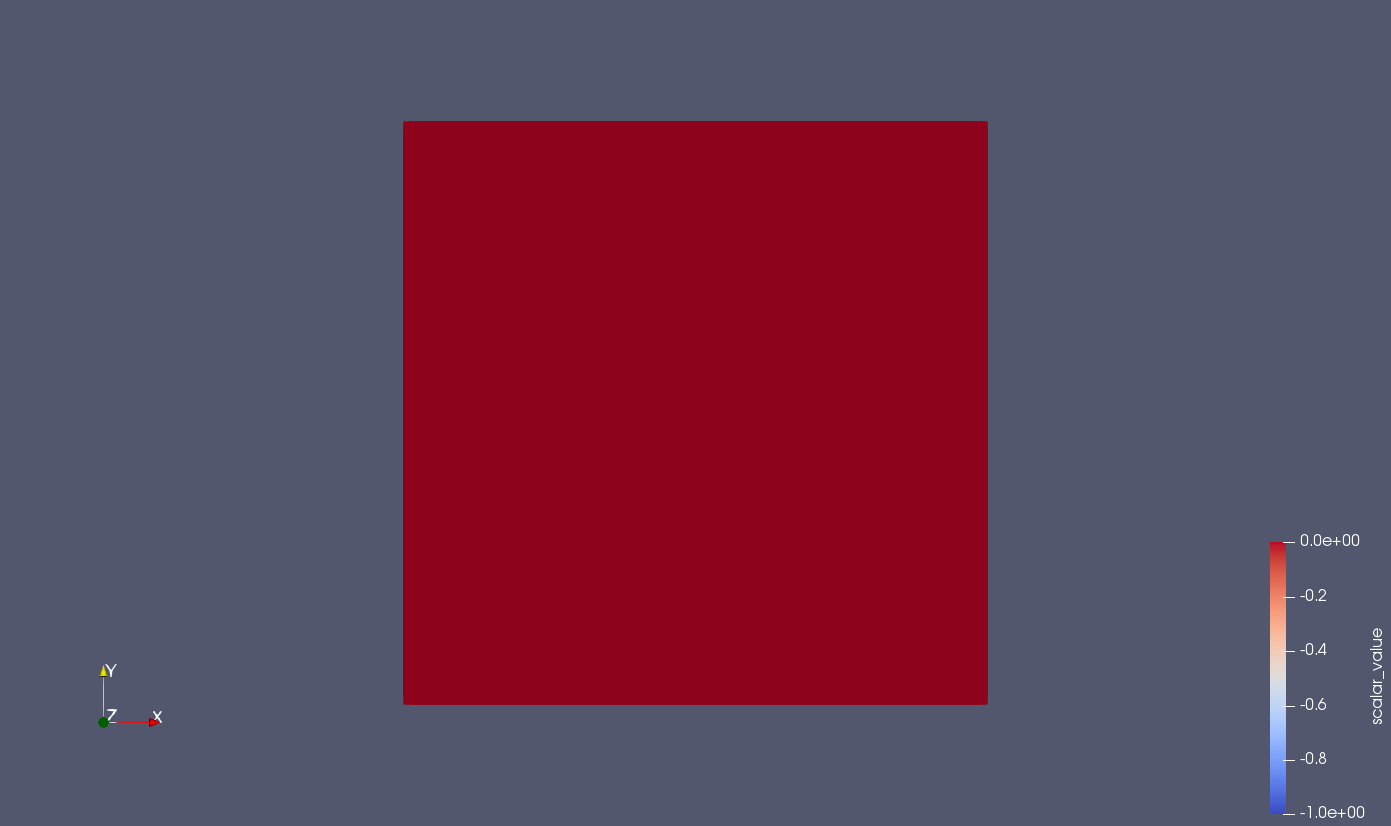
\includegraphics[width=\textwidth]{../Problem_SimpleMesh_UnitSquarelevel_8/perm.png}
%\end{figure} 
%
%\begin{figure}[H]
%	\centering
%	\captionabove{Permeabilität bei Discontinuous:}
%		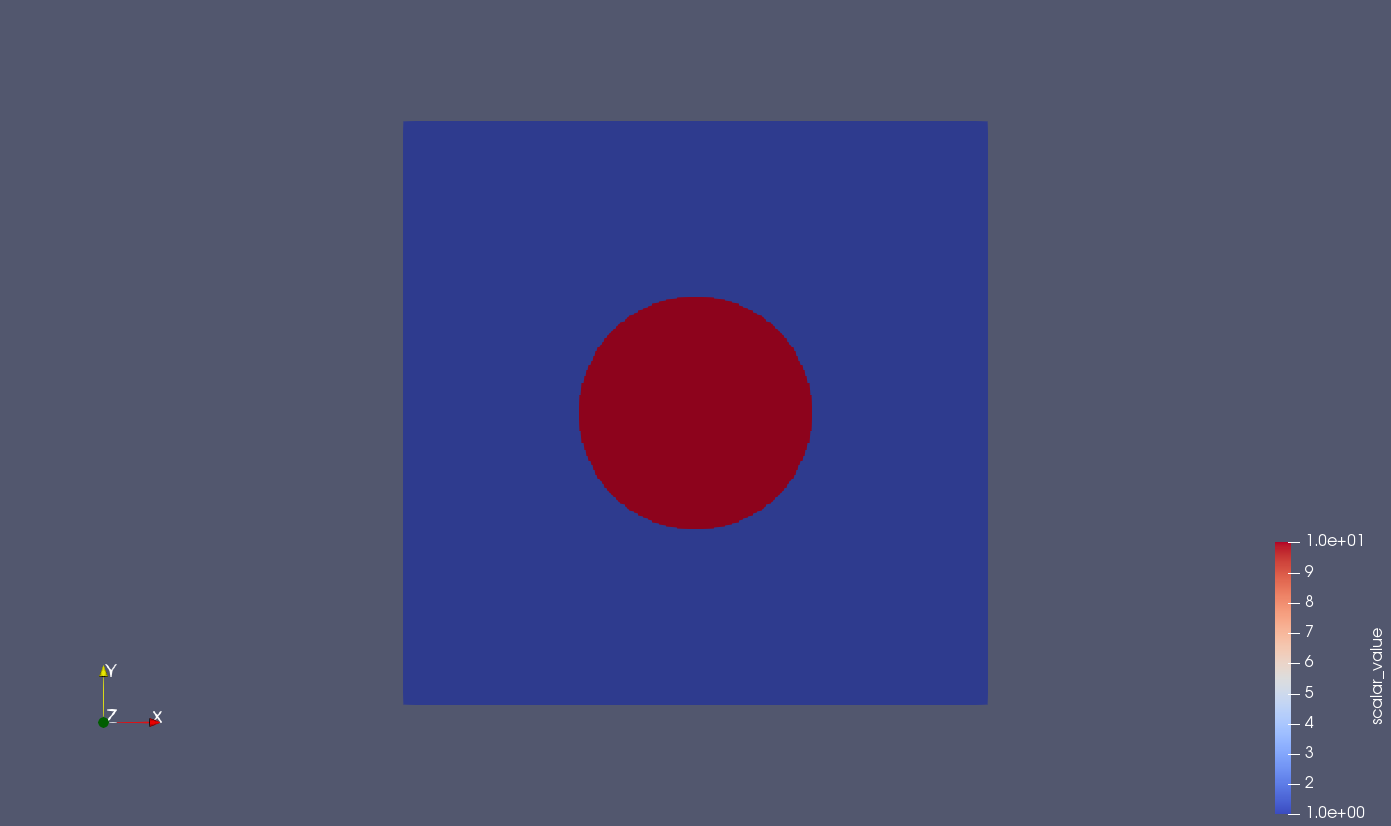
\includegraphics[width=\textwidth]{../Problem_DiscontinousMesh_UnitSquarelevel_8/perm.png}
%\end{figure}
Anhand der beiden obigen Plots lässt sich gut die kreisförmige zehnfache Permeabilität in der Mitte des Gebietes beim Problem Discontinuous erkennen. 
\newline

\begin{figure}[H]
	\centering
	\captionabove{u bei Simple und bei Discontinuous}
	\subfigure[Problem Simple]{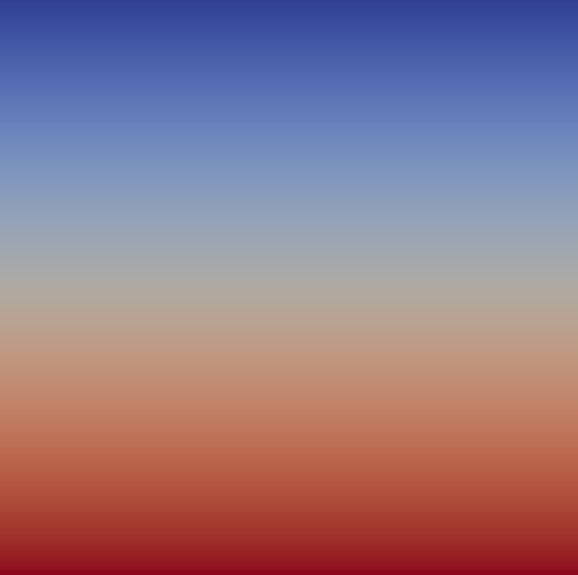
\includegraphics[width=0.49\textwidth]{../Problem_SimpleMesh_UnitSquarelevel_8/u_geschnitten.png}}	 
	\subfigure[Problem Discontinuous]{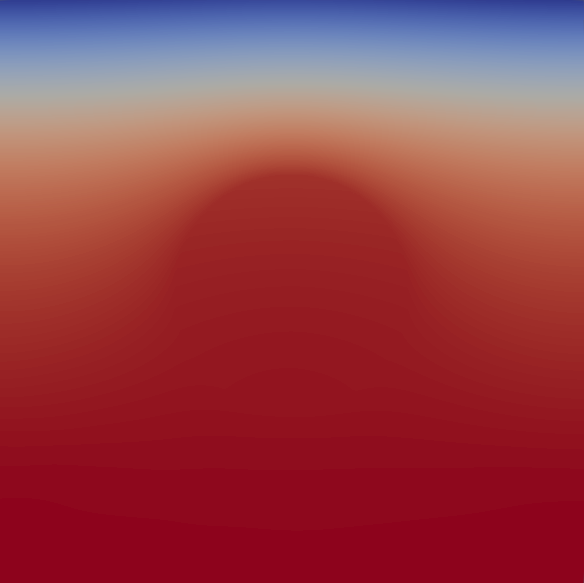
\includegraphics[width=0.49\textwidth]{../Problem_DiscontinousMesh_UnitSquarelevel_8/u2.png}}	
\end{figure}

%\begin{figure}[H]
%	\centering
%	\captionabove{u bei Simple:}
% 		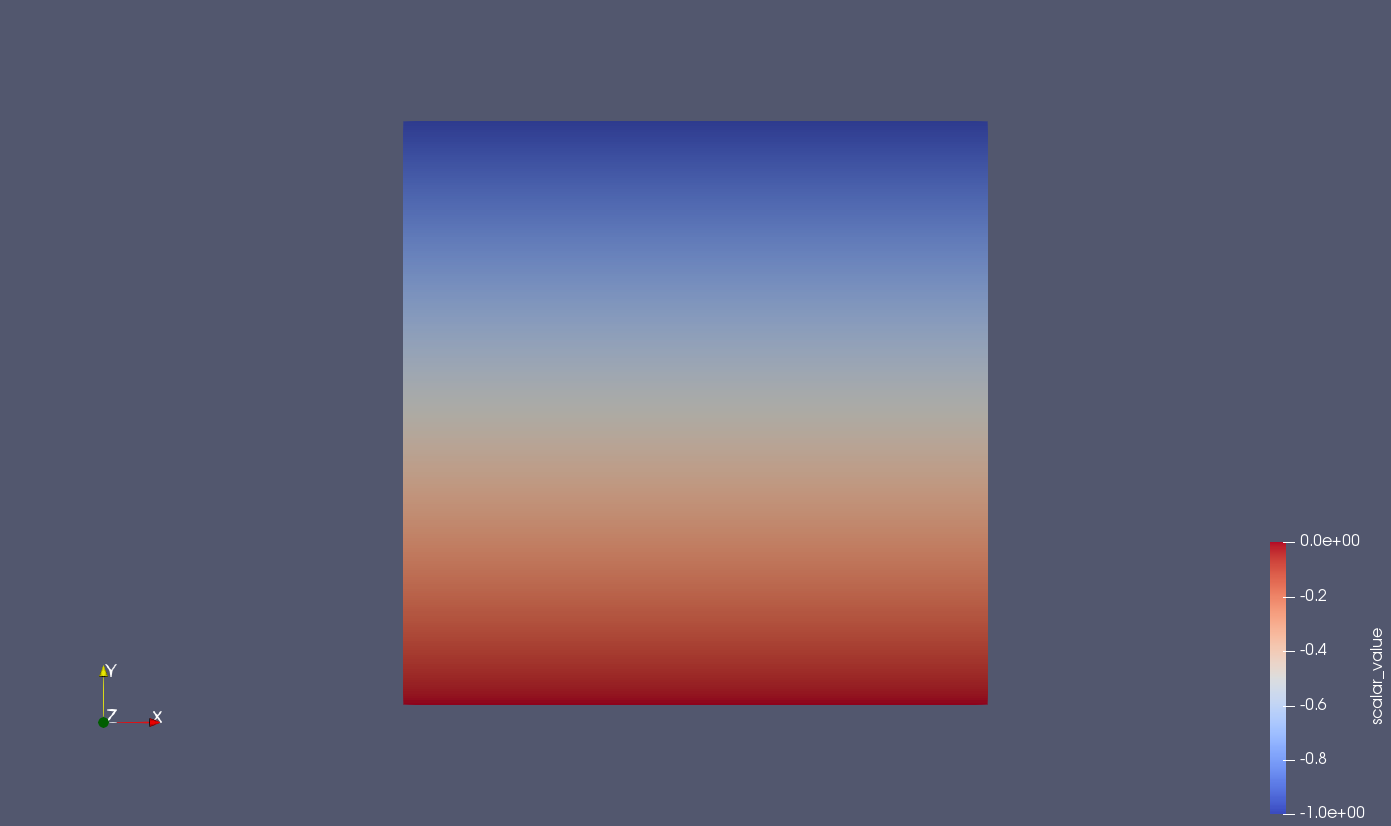
\includegraphics[width=\textwidth]{../Problem_SimpleMesh_UnitSquarelevel_8/u.png} 
%\end{figure}
%
%\begin{figure}[H]
%	\centering
%	\captionabove{u bei Discontinuous:}
%	 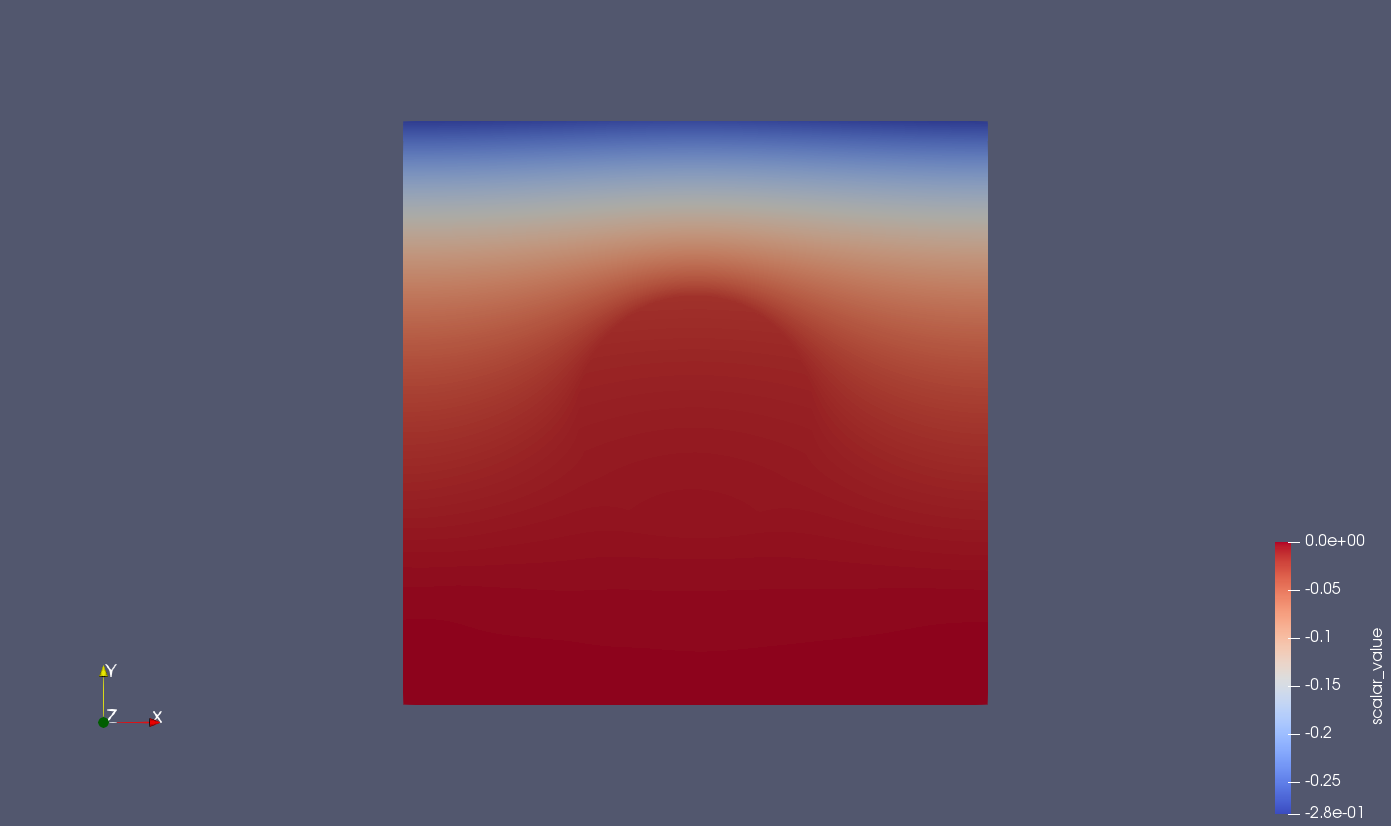
\includegraphics[width=\textwidth]{../Problem_DiscontinousMesh_UnitSquarelevel_8/u.png}
%\end{figure} 
Der Einfluss der erhöhten Permeabilität bei dem Problem Discontinuous ergibt deutlich niedrigere Werte des Potenziales u in der Mitte des Gebietes. Dadurch wird das Fluid versuchen, durch dieses zu fließen (siehe Bild Aufgabe 6, 4.3).
\begin{figure}[H]
	\centering
	\captionabove{}
	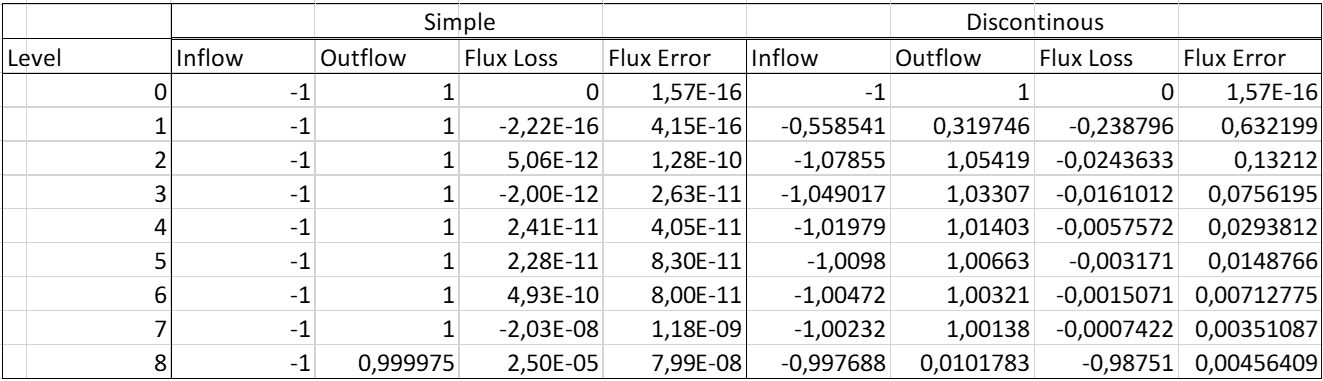
\includegraphics[width=\textwidth]{../A4Tabelle.png}
\end{figure}
Anhand der Tabelle wird deutlich, dass das Problem Simple auf allen Levels gut gelöst wird, da der Flux Error immer sehr niedrig ist. Der Fehler (Flux Error) fällt hierbei trotz höheren Levels teilweise gering höher aus, da aufgrund der größeren Komplexität vermehrt Rechenfehler im Bereich der Maschinengenauigkeit auftreten und sich aufsummieren. 
\newline Beim Problem Discontinuous halbiert sich der Fehler hingegen jeweils pro Level (von Level 2-7)
 annähernd. Die Werte bei Level 8 sind hingegen sehr verwunderlich. Zu Erwarten war hier auch eine Halbierung des Fehlers. \newline
Einstellungen hier waren$:$
\newline
 Model $=$ Laplace, Mesh $=$ UnitSquare, Overlap $=$ dG1,
  disc dG vector $=$
dGvector transport P1, Discretization $=$ linear,
  Distribution $=$ RCB, level $=$ 8, plevel $=$ 7, SetSolution $=$ 0, penalty $=$ 100000, brickearth $=$ 1, LinearSolver $=$ GMRES, Preconditioner $=$ GaussSeidel
Transfer = MatrixTransfer, 
presmoothing = 5, 
postsmoothing = 5, 
SmootherDamp = 0.8, 
Smoother = SGS, 
BasePreconditioner = LIB PS, 
BaseSolver = LS, 
TimeLevel = 0, 
vtkplot = 1, 
LinearReduction = 1e-20, 
LinearEpsilon = 1e-10, 
LinearSteps = 1000, 
LinearVerbose = 0, 
BaseSolverVerbose = -1, 
NewtonVerbose = 1, 
NewtonSteps = 100, 
NewtonLineSearchSteps = 3 und 
DebugLevel = 1.
\newline 
Die Ergebnisse ändern sich nicht, wenn eine andere Prozessorzahl gewählt wird. Die Rechnung an sich bleibt die Gleiche, bloß die Ausführungsreihenfolge bzw. die Parallelisierung ändern sich je nach Anzahl der benutzten Prozesse. 

\item Aufgabe 6
\newline
1. Geometrien
\newline


\begin{figure}[H]
	\centering
	\captionabove{Geometrien}
	\subfigure[Mesh 'UnitSquare8Triangels' auf Level 3]{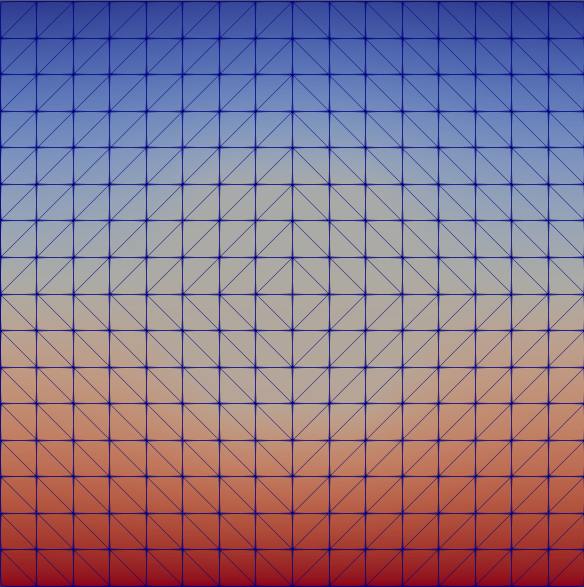
\includegraphics[width=0.49\textwidth]{../Aufgabe6/Problem_Discontinuous/Mesh_UnitSquare8Triangles/level_3/geometrie2.png}}	 
	\subfigure[Mesh 'UnitSquare500' auf Level 0]{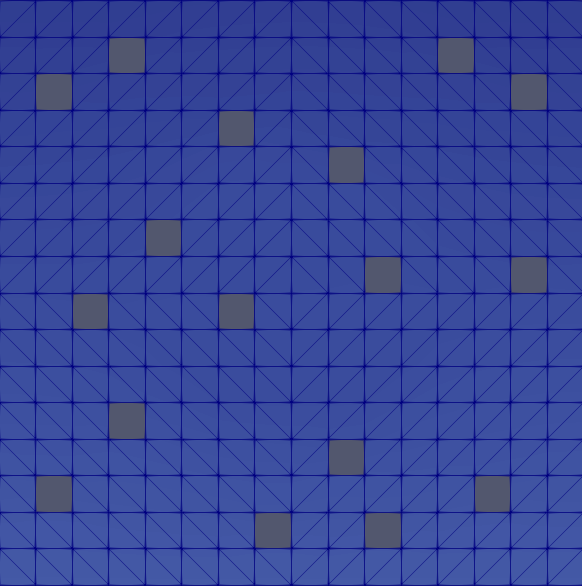
\includegraphics[width=0.49\textwidth]{../Aufgabe6/Problem_Discontinuous/Mash_Square500/level_0/geometrie2.png}}	
\end{figure}

%\begin{figure}[H]
%	\centering
%	\captionabove{Geometrie des Mesh 'UnitSquare8Triangels' auf Level 3}
%		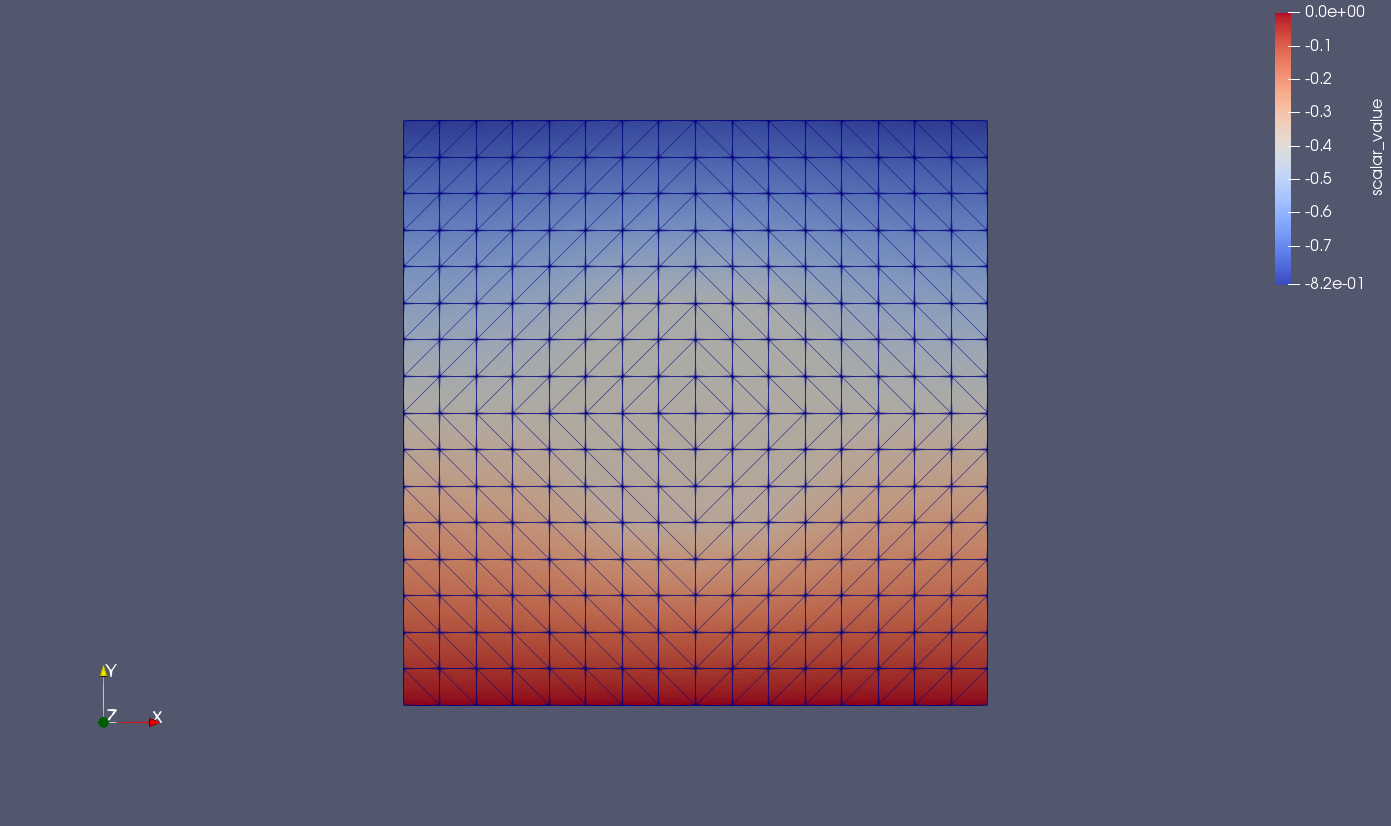
\includegraphics[width=\textwidth]{../Aufgabe6/Problem_Discontinuous/Mesh_UnitSquare8Triangles/level_3/geometrie.png} 
%\end{figure}
%
%\begin{figure}[H]
%	\centering
%	\captionabove{Geometrie des Mesh 'UnitSquare500' auf Level 0}
%		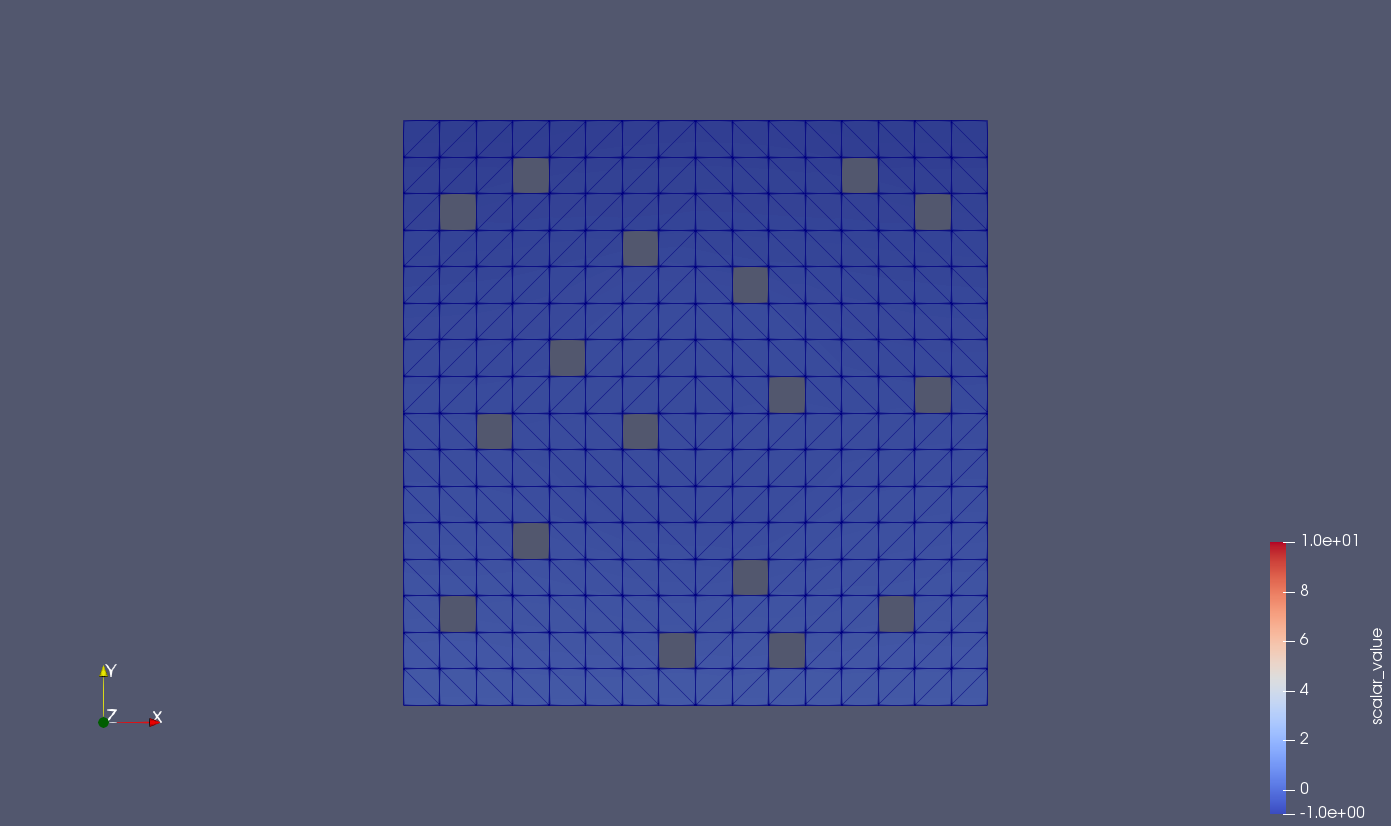
\includegraphics[width=\textwidth]{../Aufgabe6/Problem_Discontinuous/Mash_Square500/level_0/geometrie.png} 
%\end{figure}

2. Aufteilung der Rechenlast

\begin{figure}[H]
	\centering
	\captionabove{Aufteilung der Gebiete auf 4 Prozessoren}
	\subfigure[Mesh 'UnitSquare8Triangels' auf Level 3]{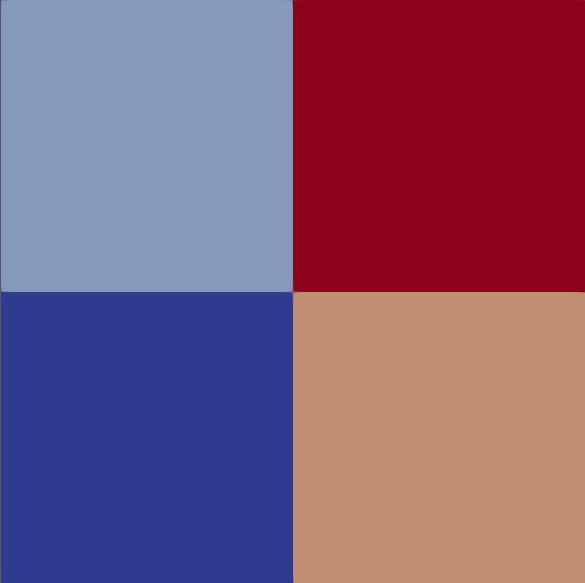
\includegraphics[width=0.49\textwidth]{../Aufgabe6/Problem_Discontinuous/Mesh_UnitSquare8Triangles/level_3/process2.png}}	 
	\subfigure[Mesh 'UnitSquare500' auf Level 0]{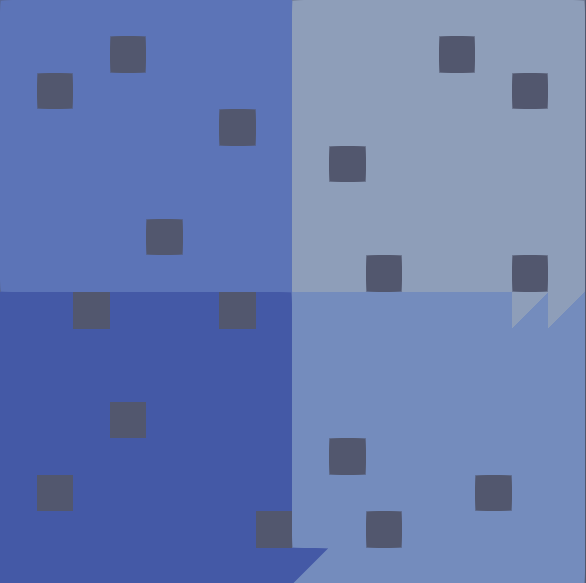
\includegraphics[width=0.49\textwidth]{../Aufgabe6/Problem_Discontinuous/Mash_Square500/level_0/process2.png}}	
\end{figure}


%\begin{figure}[H]
%	\centering
%	\captionabove{Aufteilung der Gebiete auf 4 Prozessoren des Mesh 'UnitSquare8Triangels' auf Level 3}
%		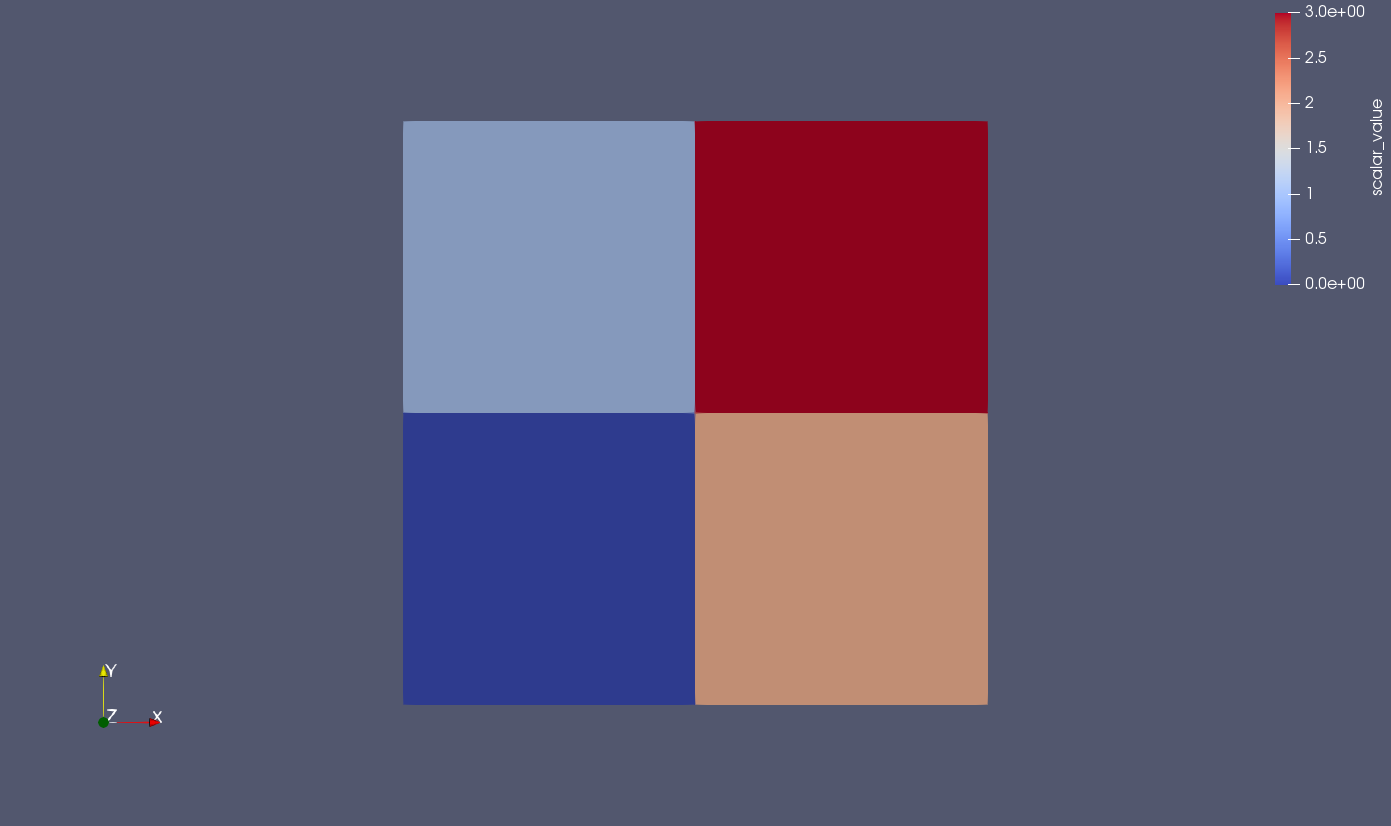
\includegraphics[width=\textwidth]{../Aufgabe6/Problem_Discontinuous/Mesh_UnitSquare8Triangles/level_3/process.png} 
%\end{figure}
%
%
%\begin{figure}[H]
%	\centering
%	\captionabove{Aufteilung der Gebiete auf 4 Prozessoren des Mesh 'UnitSquare500' auf Level 0}
%		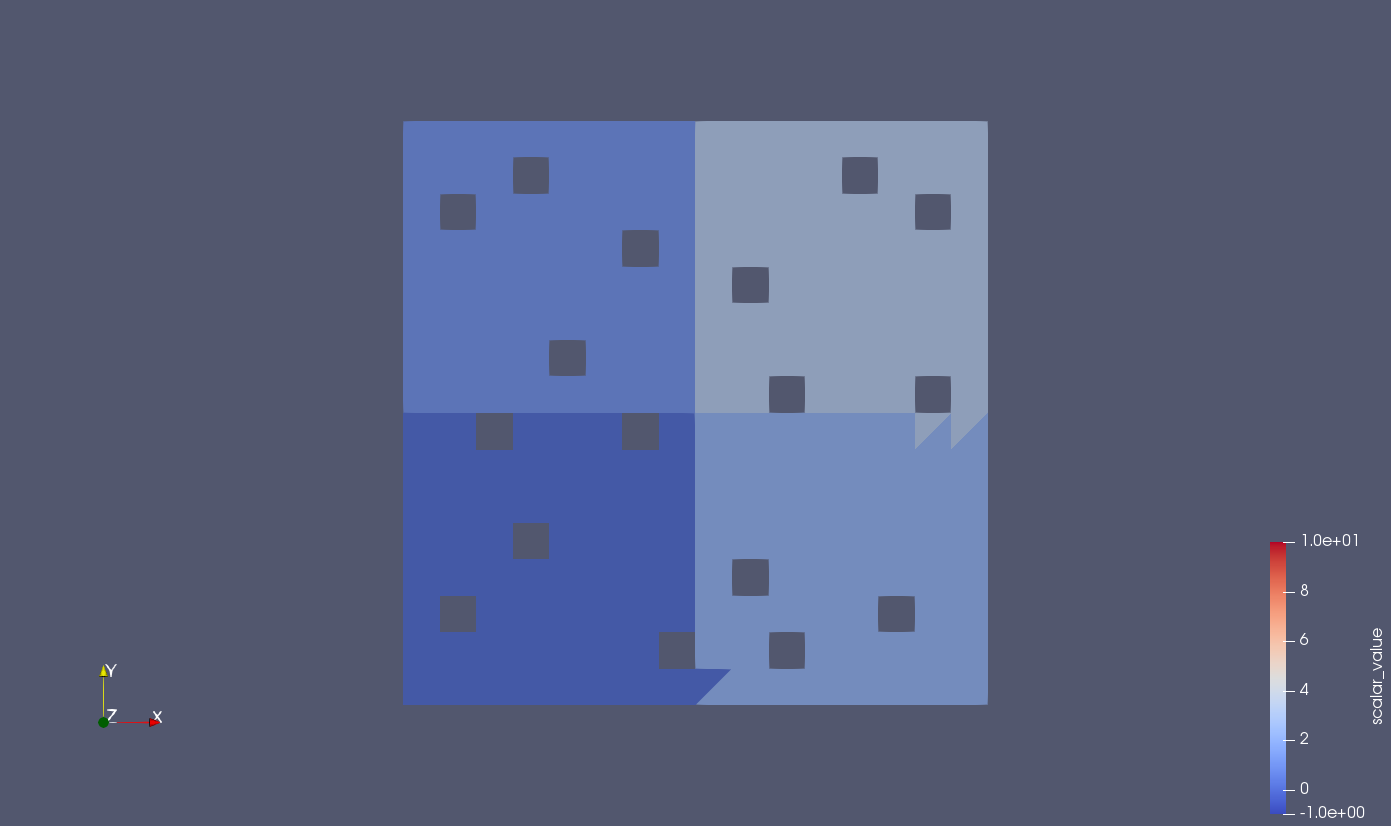
\includegraphics[width=\textwidth]{../Aufgabe6/Problem_Discontinuous/Mash_Square500/level_0/process.png} 
%\end{figure}
Man sieht gerade bei Abbildung 9 b) sehr schön, dass die Rechenlast gleichmäßig auf die 4 Prozessoren verteilt wird, indem Gebiete mit mehr 'Löchern' einzelne Zellen benachbarter Gebiete übernehmen. \newline


\begin{figure}[H]
	\centering
	\captionabove{Permeabilitäten der Probleme Simple und Discontinuous}
	\subfigure[Problem Simple auf Mesh 'UnitSquare8Triangels' auf Level 7]{
\includegraphics[width=0.39\textwidth]{../Problem_Simple2DMesh_UnitSquare8Triangelslevel_7/perm2.png}}	 
	\subfigure[Problem Simple auf Mesh 'UnitSquare500' auf Level 0]{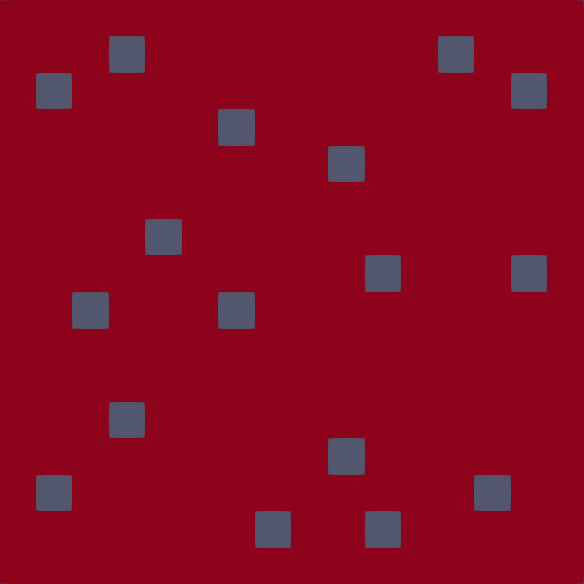
\includegraphics[width=0.39\textwidth]{../Problem_Simple2DMesh_Square500level_4/perm2.png}}	
	\subfigure[Problem Discontinuous auf Mesh 'UnitSquare8Triangels' auf Level 7]{
\includegraphics[width=0.39\textwidth]{../Problem_DiscontinousMesh_UnitSquare8Triangelslevel_7/perm2.png}}	
	\subfigure[Problem Discontinuous auf Mesh 'UnitSquare500' auf Level 0]{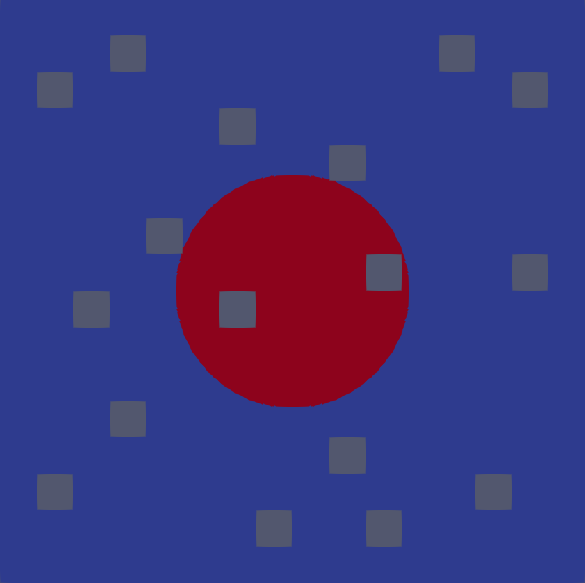
\includegraphics[width=0.39\textwidth]{../Problem_DiscontinousMesh_Square500level_4/perm2.png}}	
\end{figure}


%\begin{figure}[H]
%	\centering
%	\captionabove{Permeabilität des Problem Simple auf Mesh 'UnitSquare8Triangels' auf Level 7}
%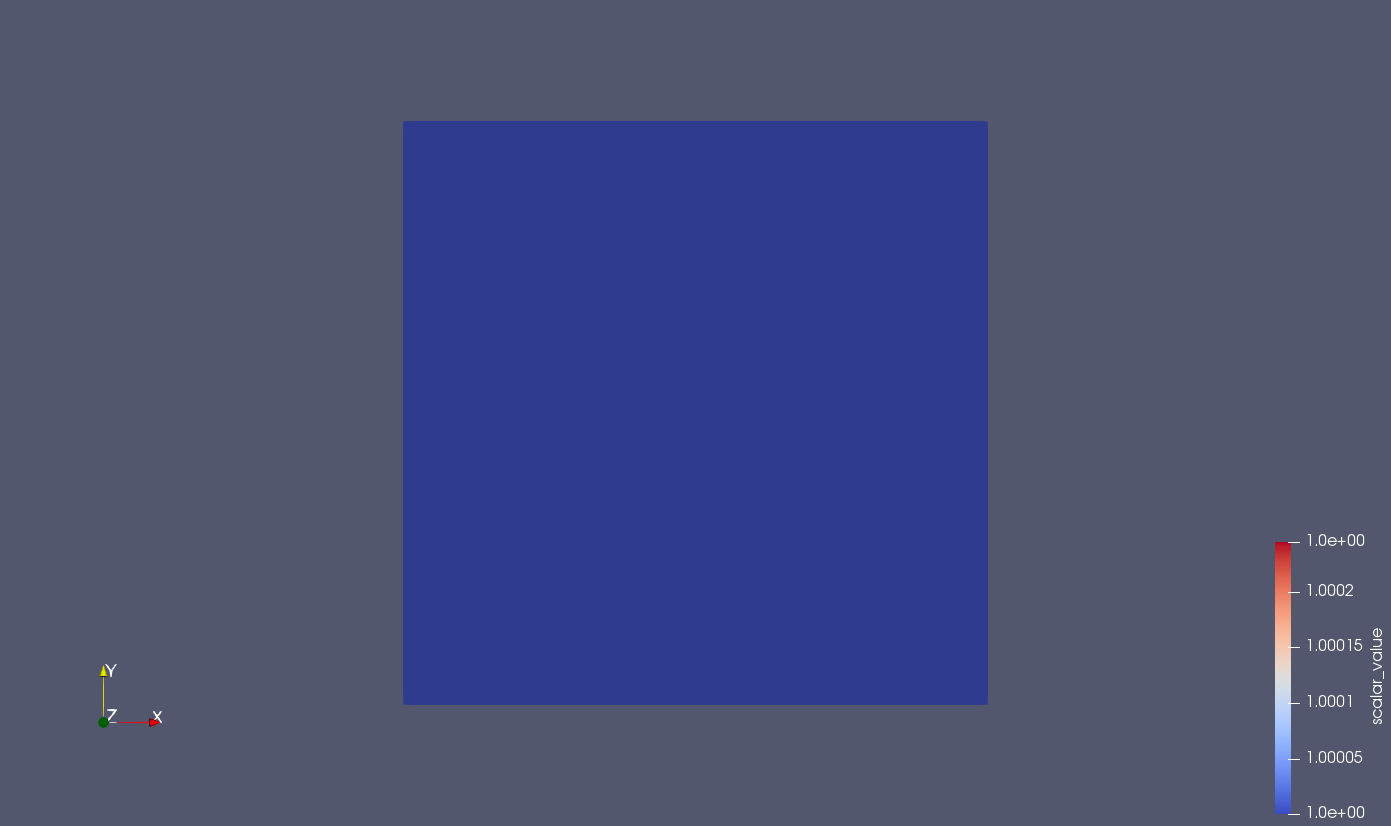
\includegraphics[width=\textwidth]{../Problem_Simple2DMesh_UnitSquare8Triangelslevel_7/perm.png} 
%\end{figure}
%
%
%\begin{figure}[H]
%	\centering
%	\captionabove{Permeabilität des Problem Simple auf Mesh 'UnitSquare500' auf Level 0}
%		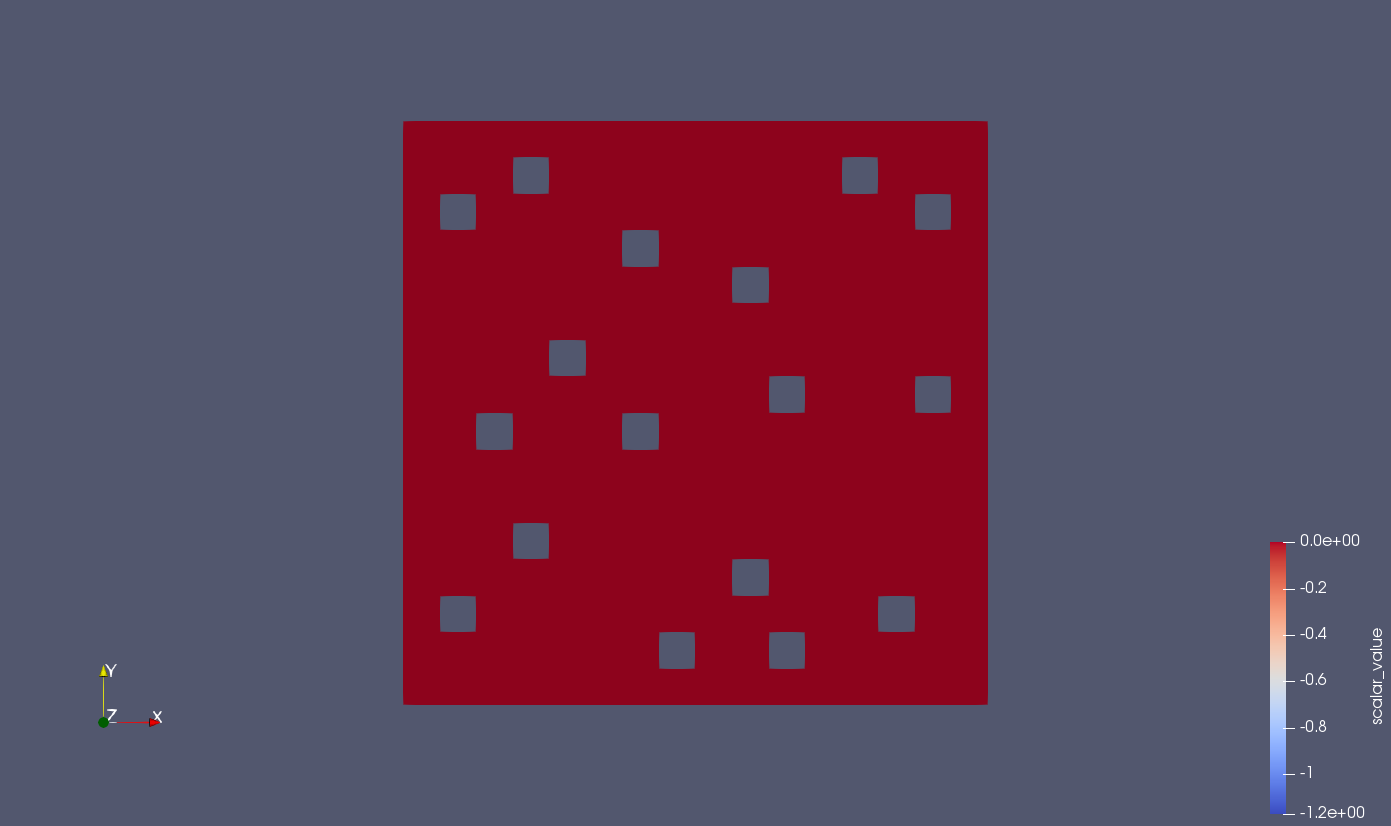
\includegraphics[width=\textwidth]{../Problem_Simple2DMesh_Square500level_4/perm.png} 
%\end{figure}
%
%
%\begin{figure}[H]
%	\centering
%	\captionabove{Permeabilität des Problem Discontinuous auf Mesh 'UnitSquare8Triangels' auf Level 7}
%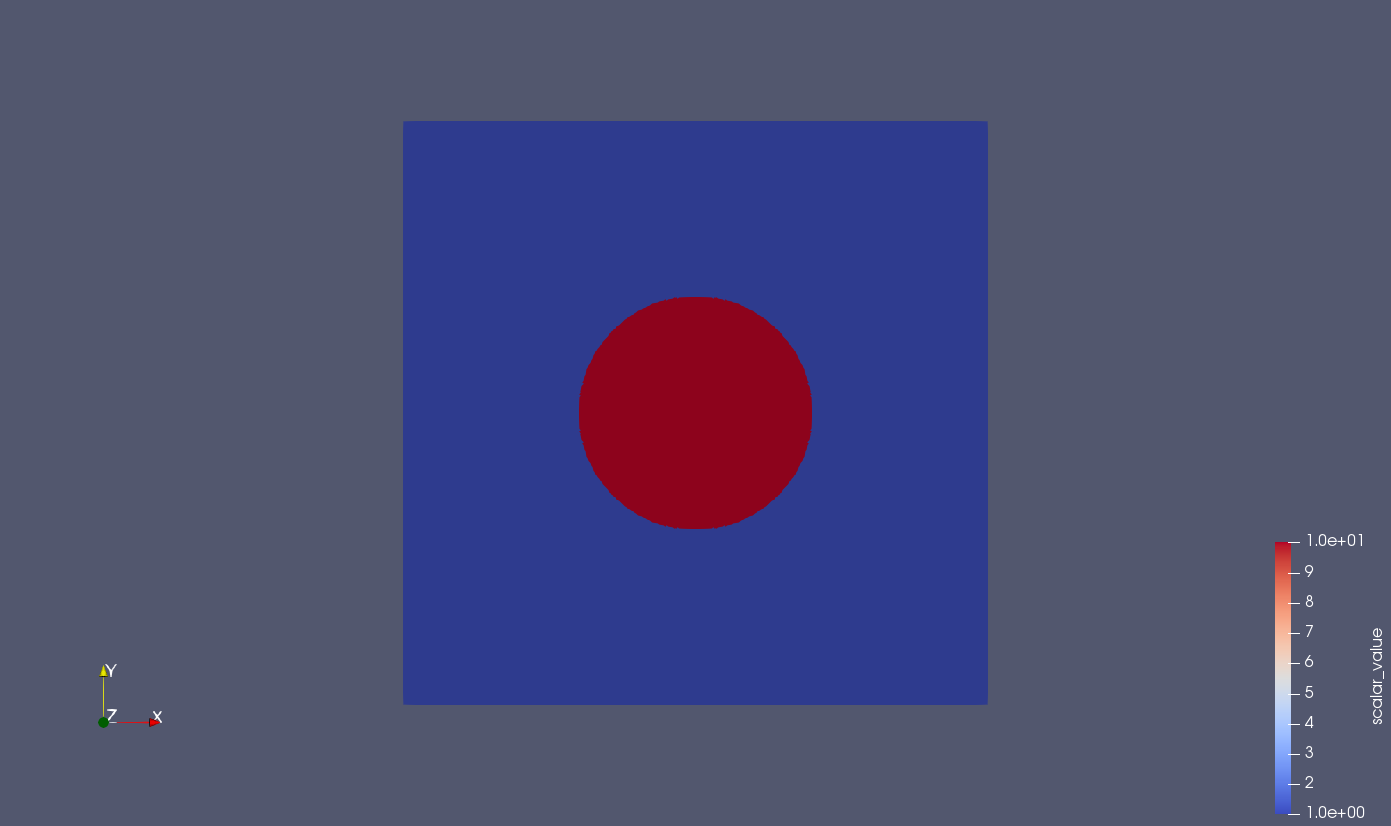
\includegraphics[width=\textwidth]{../Problem_DiscontinousMesh_UnitSquare8Triangelslevel_7/perm.png} 
%\end{figure}
%
%
%\begin{figure}[H]
%	\centering
%	\captionabove{Permeabilität des Problem Discontinuous auf Mesh 'UnitSquare500' auf Level 0}
%		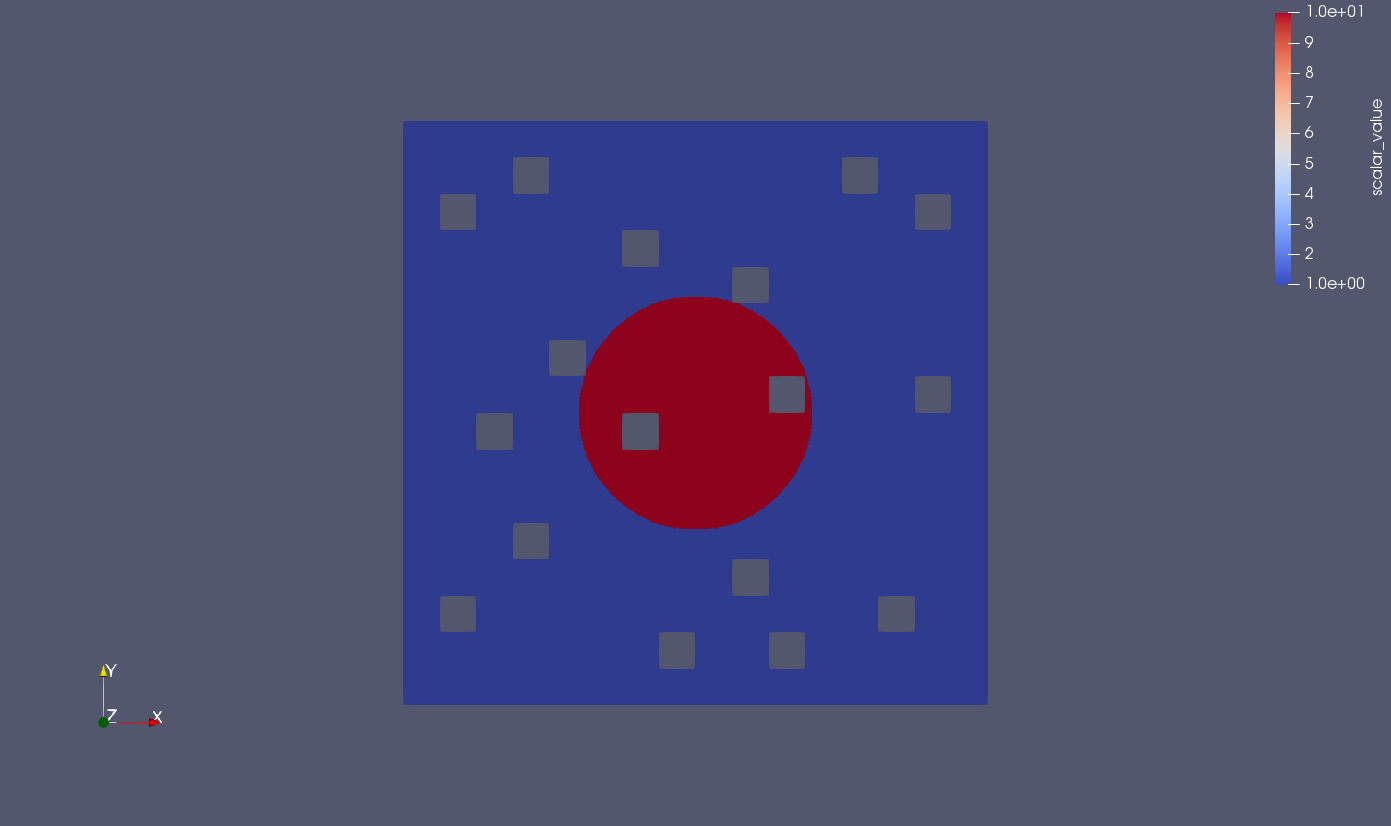
\includegraphics[width=\textwidth]{../Problem_DiscontinousMesh_Square500level_4/perm.png} 
%\end{figure}


4. Lösungen
\newline
\begin{figure}[H]
	\centering
	\captionabove{Lösungen des homogenen und inhomogenen Problems mit Strömungslinien}
	\subfigure[Problem Simple auf Mesh 'UnitSquare8Triangels' auf Level 7]{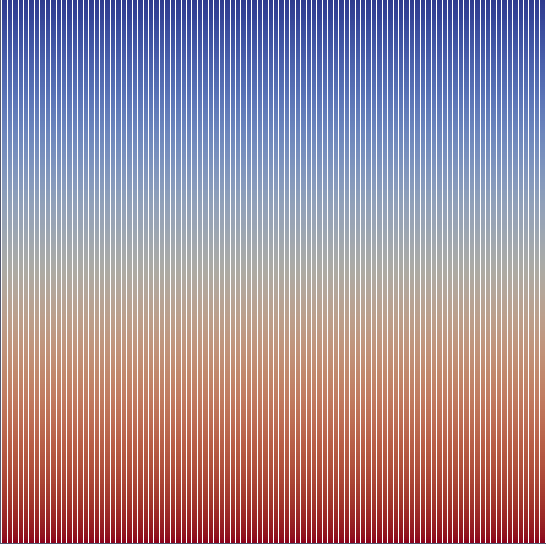
\includegraphics[width=0.49\textwidth]{../Problem_Simple2DMesh_UnitSquare8Triangelslevel_7/blub2.png}}	 
	\subfigure[Problem Simple auf Mesh 'UnitSquare500' auf Level 0]{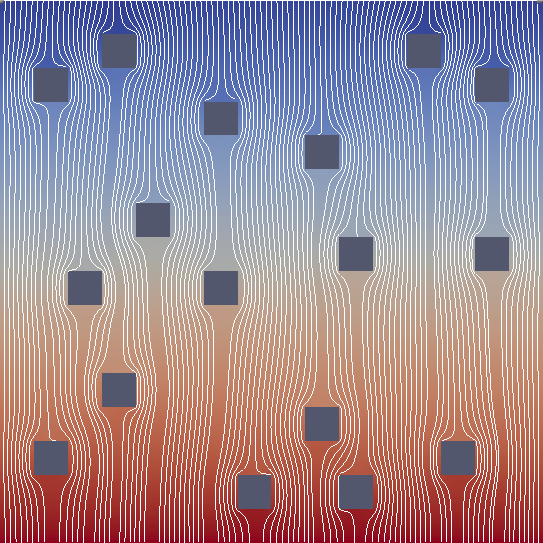
\includegraphics[width=0.49\textwidth]{../Problem_Simple2DMesh_Square500level_4/blub2.png}}	
	\subfigure[Problem Discontinuous auf Mesh 'UnitSquare8Triangels' auf Level 7]{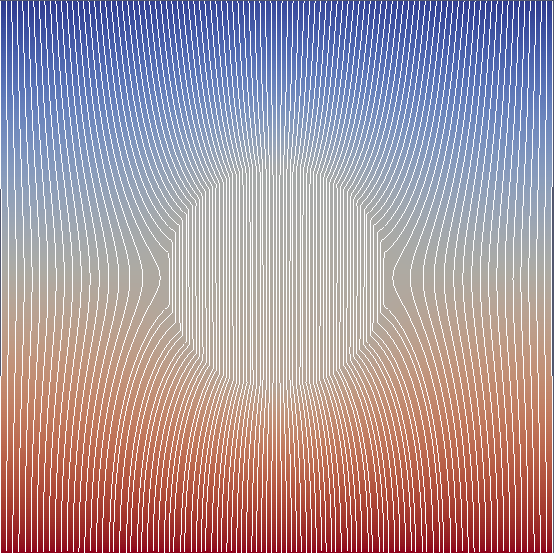
\includegraphics[width=0.49\textwidth]{../Problem_DiscontinousMesh_UnitSquare8Triangelslevel_7/blub2.png}}	
	\subfigure[Problem Discontinuous auf Mesh 'UnitSquare500' auf Level 0]{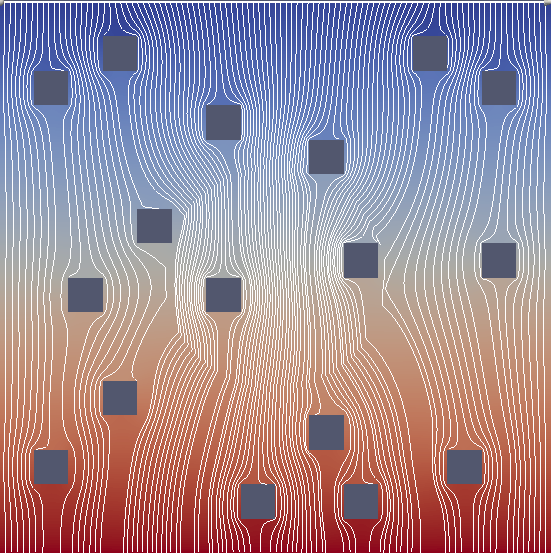
\includegraphics[width=0.49\textwidth]{../Problem_DiscontinousMesh_Square500level_4/blub2.png}}	
\end{figure}

%\begin{figure}[H]
%	\centering
%	\captionabove{Lösung zum homogenen Problem auf dem Mesh 'UnitSquare8Triangels' mit Strömungslinien auf Level 7}
%		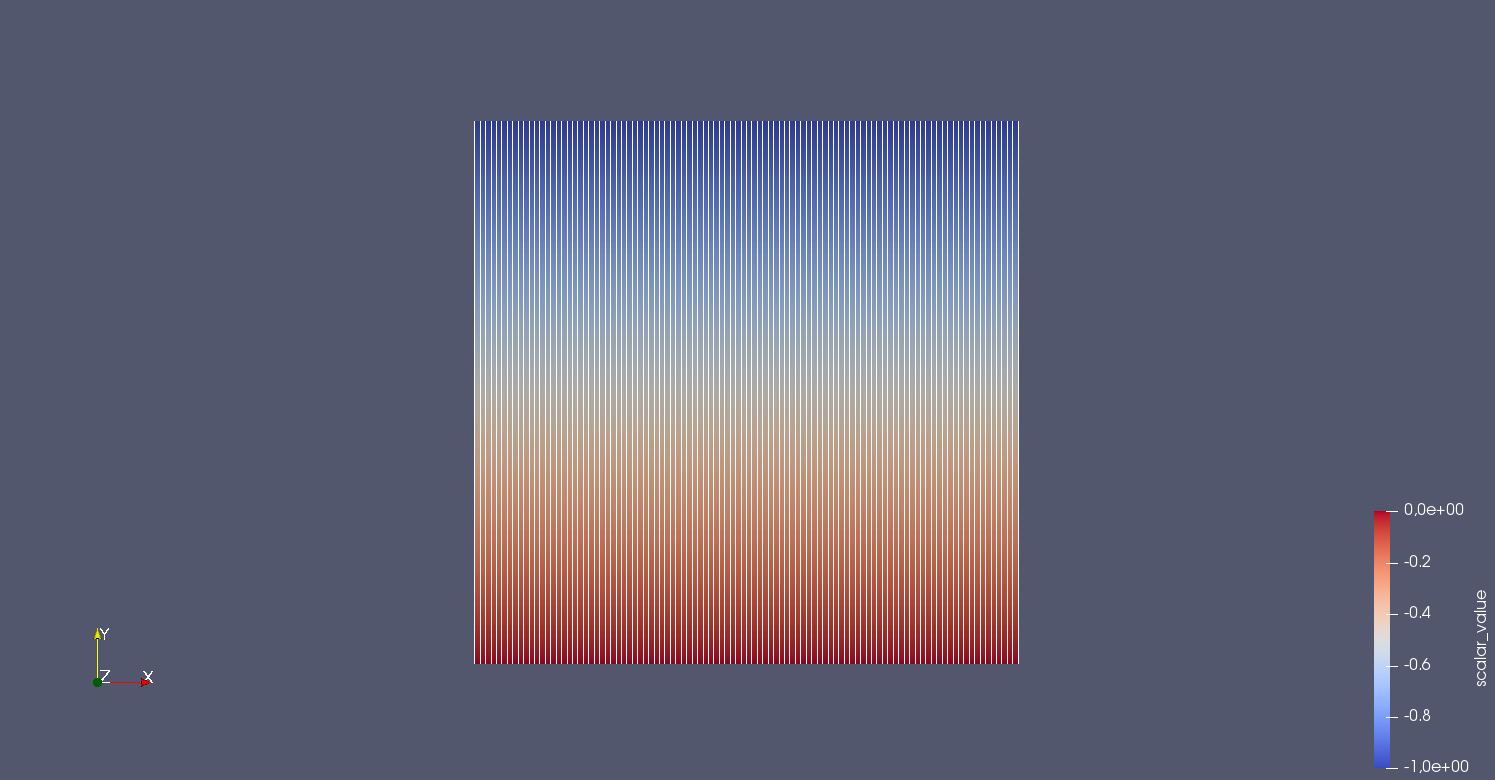
\includegraphics[width=\textwidth]{../Problem_Simple2DMesh_UnitSquare8Triangelslevel_7/blub.png} 
%\end{figure}
%
%\begin{figure}[H]
%	\centering
%	\captionabove{
%Lösung zum homogenen Problem auf dem Mesh 'Square500' mit Strömungslinien auf Level 4}
%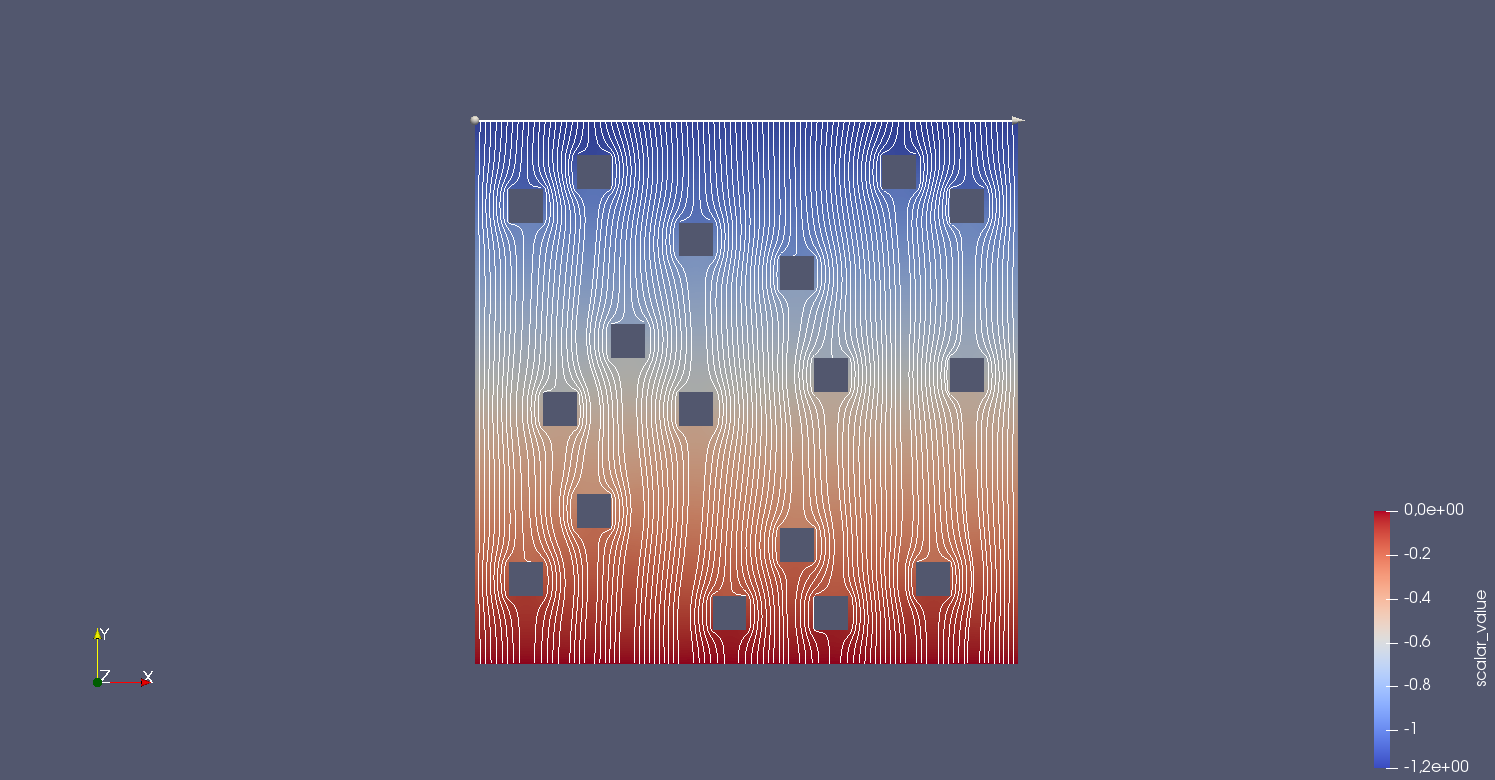
\includegraphics[width=\textwidth]{../Problem_Simple2DMesh_Square500level_4/blub.png} 
%\end{figure}
%
%\begin{figure}[H]
%	\centering
%	\captionabove{Lösung zum inhomogenen Problem auf dem Mesh 'UnitSquare8Triangels' mit Strömungslinien auf Level 7}
%		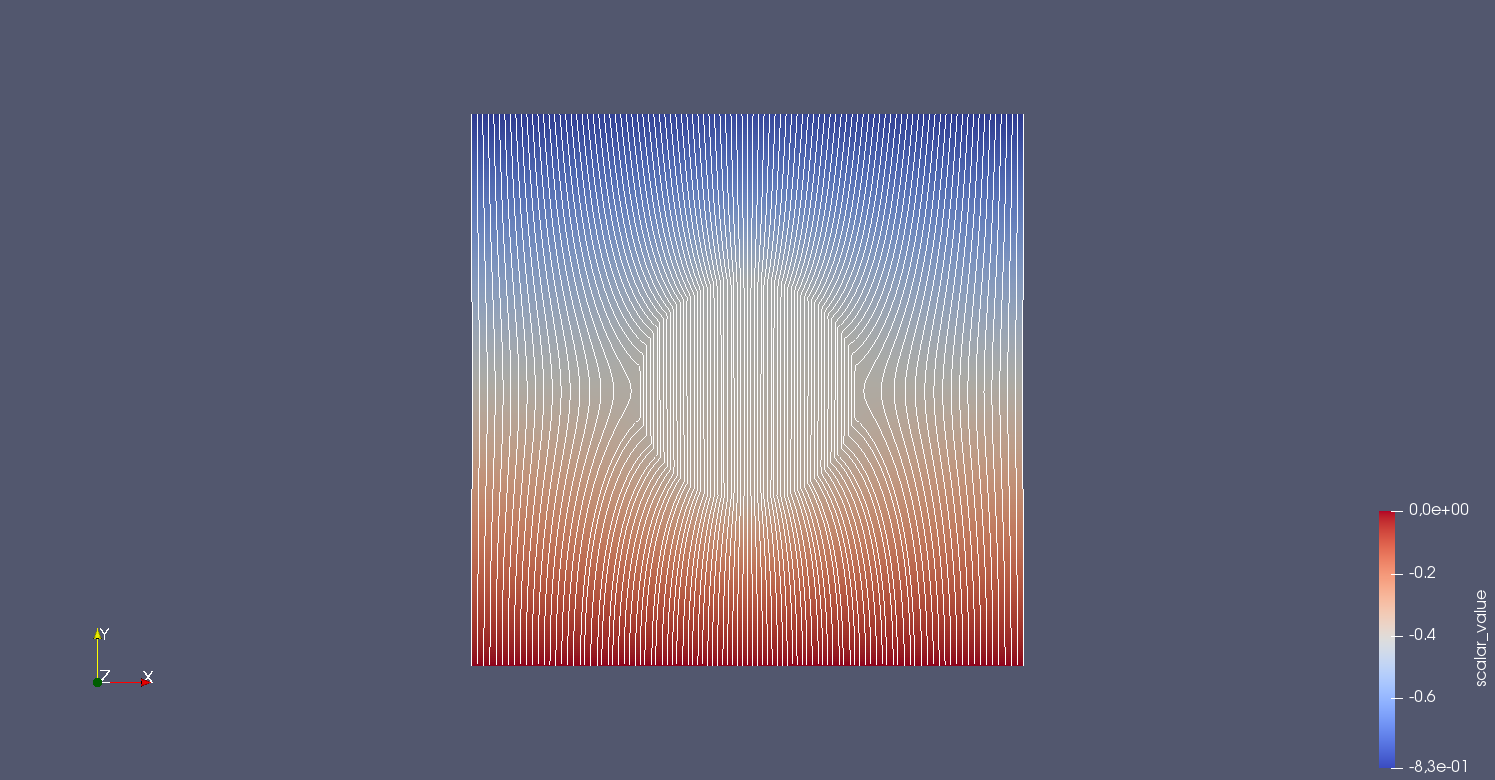
\includegraphics[width=\textwidth]{../Problem_DiscontinousMesh_UnitSquare8Triangelslevel_7/blub.png} 
%\end{figure}
%
%\begin{figure}[H]
%	\centering
%	\captionabove{Lösung zum inhomogenen Problem auf dem Mesh 'Square500' mit Strömungslinien auf Level 4}
%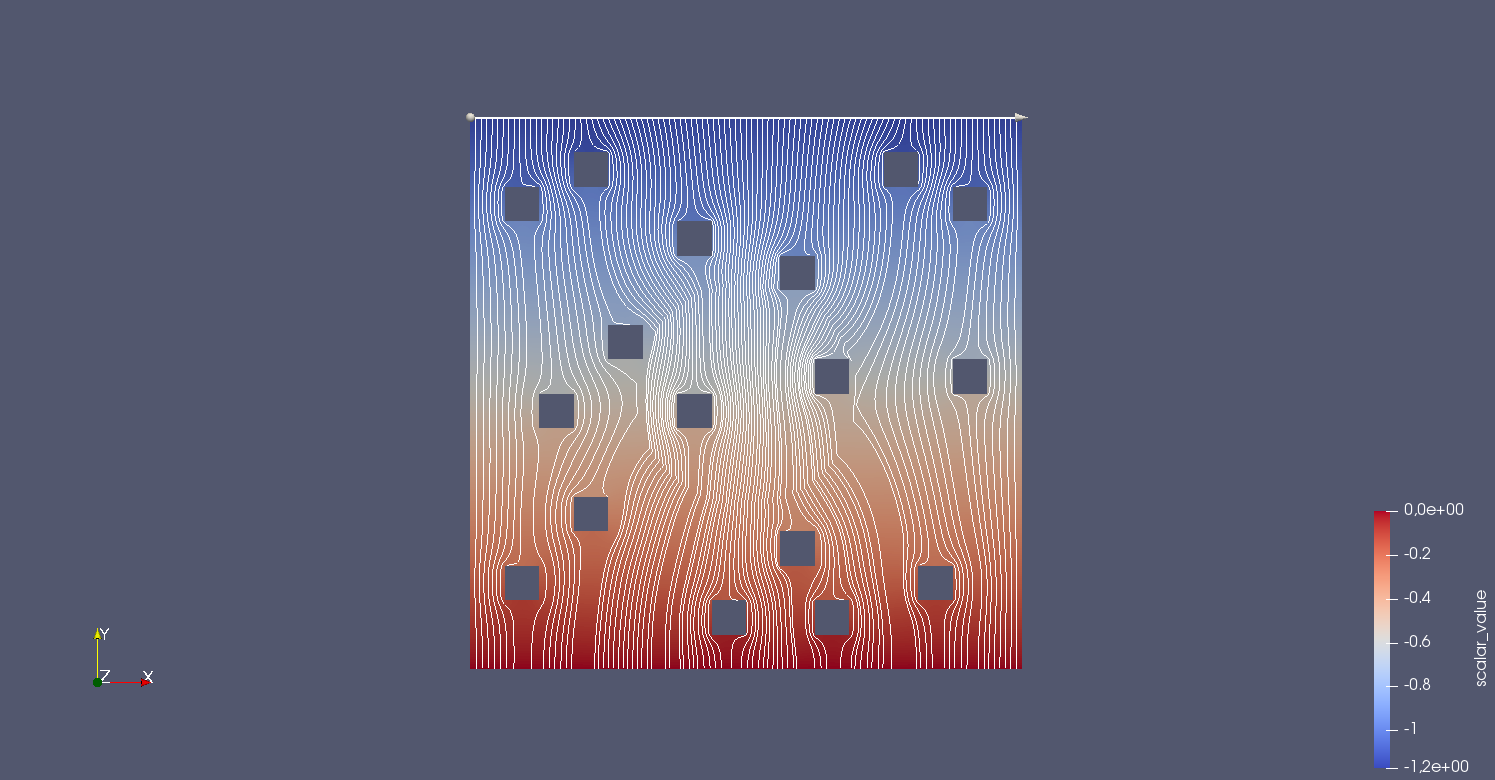
\includegraphics[width=\textwidth]{../Problem_DiscontinousMesh_Square500level_4/blub.png} 
%\end{figure}



\begin{figure}[H]
	\centering
	\captionabove{Tabelle zu 5. und 6.}
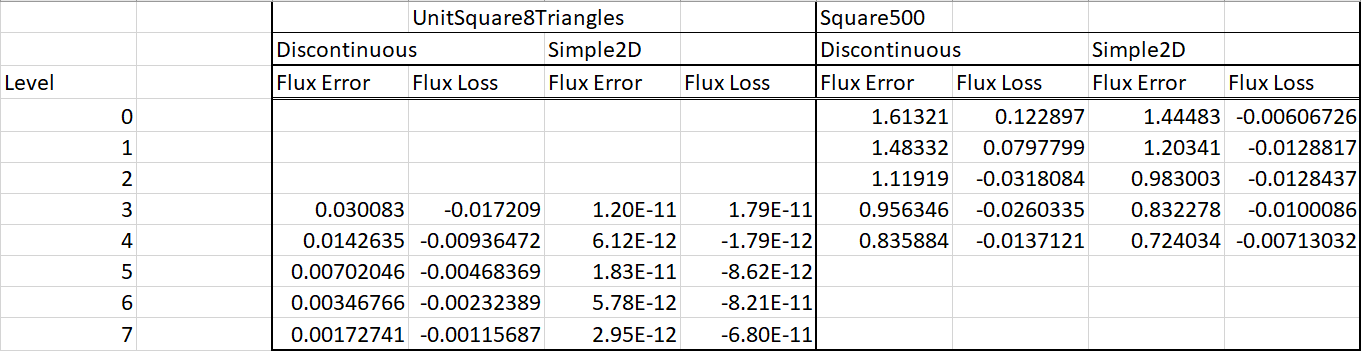
\includegraphics[width=\textwidth]{../Aufgabe6/Aufgabe6Tabelle.png}
\end{figure}

7. Interpretation \newline
Betrachten wir zunächst die Probleme auf dem Mesh 'UnitSquare8Triangels': \newline
Ähnlich wie in Aufgabe 4 sind die Fehlerwerte bei dem einfachen Problem sehr klein und es lässt sich dadurch eigentlich keine wirkliche Entwicklung ablesen. Genauso sieht man auch bei Discontinuous sehr schön die Halbierung der Fehlerwerte (insbesondere Flux Error). Insgesamt lässt so über 
\begin{align*}
h_l = h_0 \cdot 2^{-l} \text{ und } \frac{e_l}{e_{l+1}} \sim \frac{(2^{-l}h_0)^{p}}{(2^{-(l+1)}h_0)^{p}} %= \left(\frac{h_l}{h_{l+1}}\right)^p
\end{align*}
die Konvergenzrate p bestimmen. Dabei ist $l$ das Level, $h_l$ die Gitterweite, $e_l$ der Fehler auf Level l (bei uns der Flux Error). 
Bei obigen Werten erhält man $ \frac{e_l}{e_{l+1}} \approx 2.043 $. \newline
Dabei ergibt sich die Konvergenzrate $p \approx 1.03$ .
Man kann unter theoretischem Hintergrund zeigen, dass der Flux Error äquivalent zu einer Sobolevnorm ist, die genaueren Hintergründe sollen hier aber nicht Teil des Berichtes sein.

Betrachten wir nun die Probleme auf dem Mesh 'Square500': Schnell fällt auf, dass unabhängig vom gewählten Problem die Fehlerwerte um ein Vielfaches größer sind. Die deutlich schlechteren Fehlerwerte spiegeln sich auch in der (approximativen) Konvergenzrate wieder: \newline
Für das Problem Discontinuous erhalten wir $ \frac{e_l}{e_{l+1}} \approx 1.18 $ und $p \approx 0.24$ \newline
Für das Problem Simple2D erhalten wir $ \frac{e_l}{e_{l+1}} \approx 1.19 $ und $p \approx 0.25$ \newline

Man erkennt, dass beide Probleme auf 'Square500' sehr schlecht gelöst werden.

\subsubsection{Aufgabe 7}

In Aufgabe 7 betrachteten wir die beiden heterogenen Problem 'Divergent' und 'Kellogg' unter ähnlichen Gesichtspunkten wie zuvor bereits 'Simple' und 'Discontinuous'.
\begin{figure}[H]
	\centering
	\captionabove{Problem Divergent}
	\subfigure[Geometrie und Prozessoraufteilung auf Level 3]{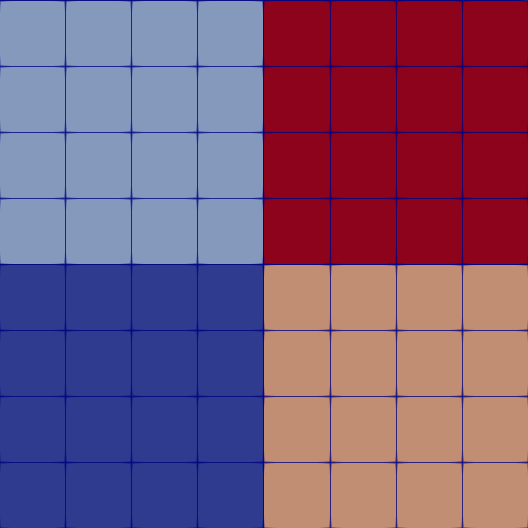
\includegraphics[width=0.39\textwidth]{../../Aufgabe7/Divergent_lvl3/geometrie.png}}	
	\subfigure[Permeabilität auf Level 3]{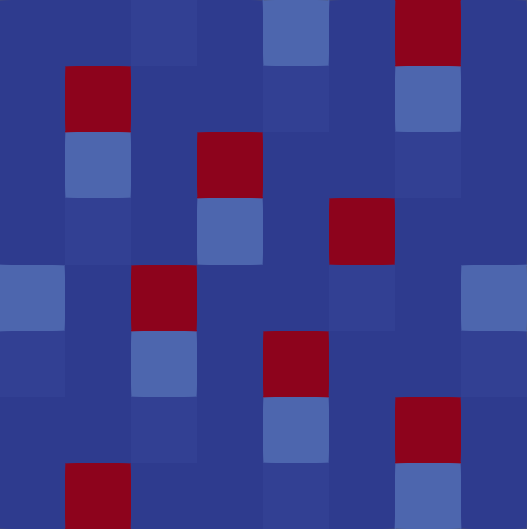
\includegraphics[width=0.39\textwidth]{../../Aufgabe7/Divergent_lvl3/perm.png}}	 
	\subfigure[Permeabilität auf Level 7]{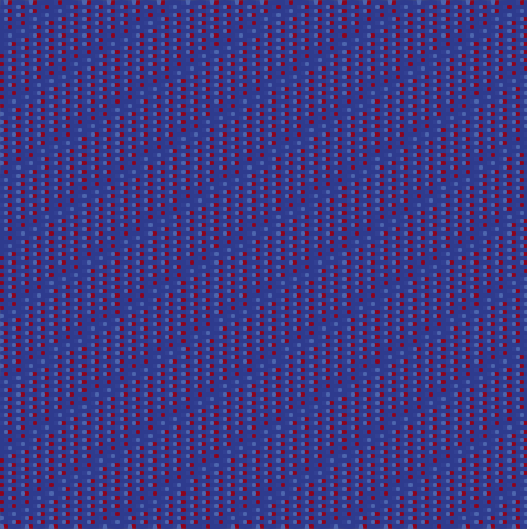
\includegraphics[width=0.39\textwidth]{../../Aufgabe7/Divergent_lvl7/perm.png}}	
	\subfigure[Lösung]{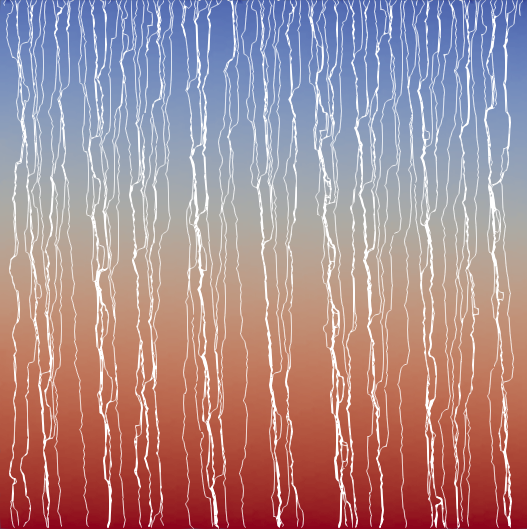
\includegraphics[width=0.39\textwidth]{../../Aufgabe7/Divergent_lvl7/u.png}}	
\end{figure}

\begin{figure}[H]
	\centering
	\captionabove{Flux Error und Flux Loss bei Problem Divergent}
	\subfigure{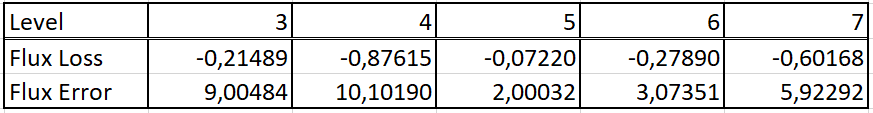
\includegraphics[width=0.99\textwidth]{../../Aufgabe7/divtabelle.png}}	 
	
\end{figure}
Beim Problem 'Divergent' erhielten wir für die Größen 'Flux Loss' und 'Flux Error' stark schwankende Ergebnisse. Es war hier insbesondere nicht wirklich möglich eine Konvergenzrate zu bestimmen. Ein Blick in die Lösungen auf unterschiedlichem Level erklärt dies:
\begin{figure}[H]
	\centering
	\captionabove{Lösungen Problem Divergent}
	\subfigure[auf Level 3]{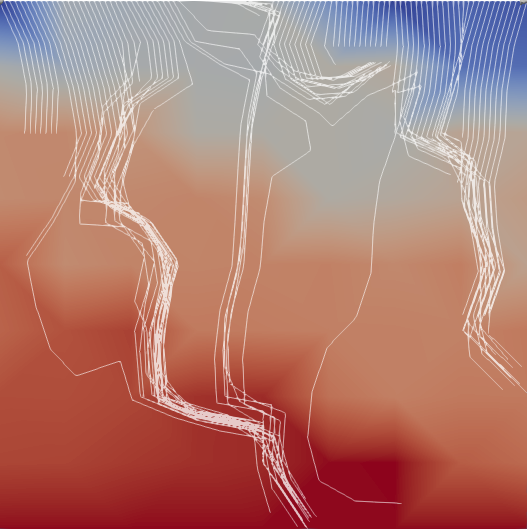
\includegraphics[width=0.30\textwidth]{../../Aufgabe7/Divergent_lvl3/u.png}}	 
	\subfigure[auf Level 5]{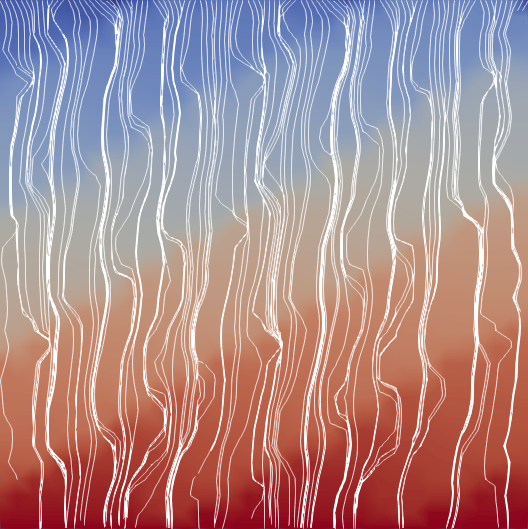
\includegraphics[width=0.30\textwidth]{../../Aufgabe7/Divergent_lvl5/u.png}}	
	\subfigure[auf Level 7]{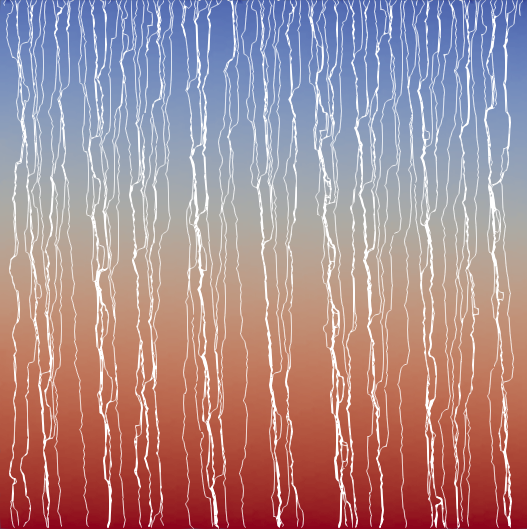
\includegraphics[width=0.30\textwidth]{../../Aufgabe7/Divergent_lvl7/u.png}}	
\end{figure}

Die Lösungen verhalten sich also auf den unterschiedlichen Leveln stark unterschiedlich, weswegen wir nicht wirklich von einer Konvergenz sprechen können.


\begin{figure}[H]
	\centering
	\captionabove{Problem Kellogg}
	\subfigure[Geometrie und Prozessoraufteilung auf Level 3]{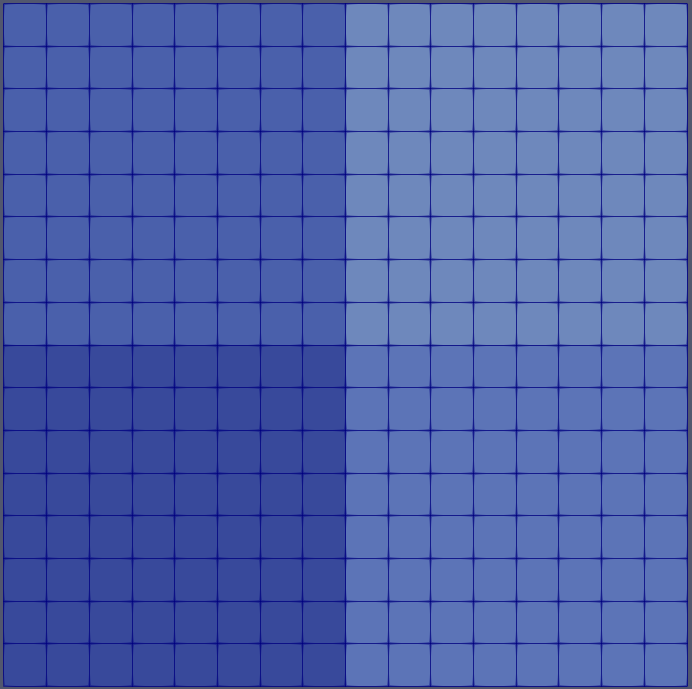
\includegraphics[width=0.39\textwidth]{../../Aufgabe7/MeshLoad.png}}	 
	\subfigure[Permeabilität auf Level 7]{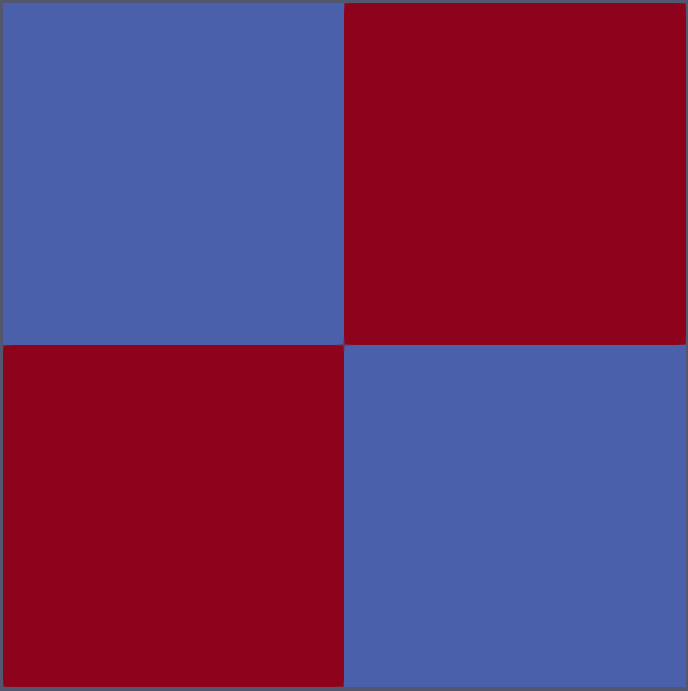
\includegraphics[width=0.39\textwidth]{../../Aufgabe7/perm.png}}	
	\subfigure[Lösung]{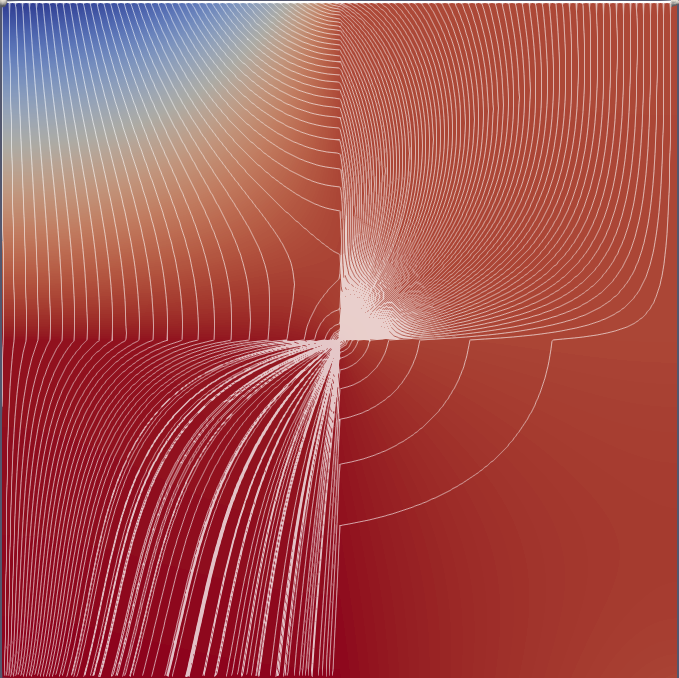
\includegraphics[width=0.39\textwidth]{../../Aufgabe7/fluss.png}}	
\end{figure}

Wie man anhand der obigen Bilder erkennen kann besteht das Problem 'Kellogg' aus einer viergeteilten Permeabilität.
Dabei haben die Gebiete rechts oben bzw. links unten eine erhöhte Durchlässigkeit.
Daraus resultiert, dass die Strömungslinien hauptsächlich durch die Mitte fliesen.

\begin{figure}[H]
	\centering
	\captionabove{Flux Error und Flux Loss bei Problem Kellogg}
	\subfigure{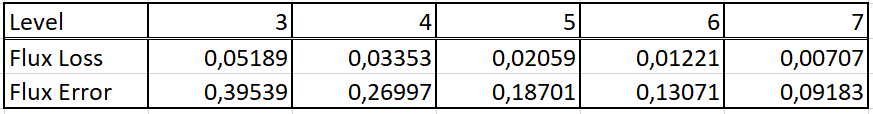
\includegraphics[width=0.99\textwidth]{../../Aufgabe7/kelltabelle.png}}	 

\end{figure}

Für das Problem 'Kellogg' erhalten wir somit $ \frac{e_l}{e_{l+1}} \approx 1.44 $ und damit die Konvergenzrate $p \approx 0.53$.

%Die 'Steine' sind in 'Square500.geo' als Löcher mit Neumann-0 Rändern innerhalb des Gebietes realisiert. 
%Betrachten wir die zugrunde liegende Differentialgleichung auf einer einzelnen Zelle der Triangulierung, erhalten wir:
%\begin{align*}
%	\begin{cases}
%		\dive q = 0 \\
%			q \cdot \nu = -g_N 
%	\end{cases}
%	\iff \int_K{ \dive q \; dx} - \int_{ \partial K}{q\cdot \nu \; da} = \int_{ \partial K \cap \Gamma_N} {g_N \; da } 
%\newline	
%\end{align*}
%In der konkreten Diskretisierung stellt sich aber für $q_h = \kappa \nabla u_h \ \in \mathbb{P}_0( \Omega_h ; \R^2) $ heraus, dass für Zellen an den Steinen gilt (Hier ist $g_h = 0$): 
%\begin{align*}	
%	 0 \neq \int_K{ \dive q_h \; dx} - \int_{ \partial K}{q_h \cdot \nu \; da} \stackrel{!}{=} \int_{ \partial K \cap \Gamma_N} {g_h \; da } = 0 
%\end{align*}
%
%Die Lösung ist also bereits für einzelne Zellen nicht korrekt, weswegen auch der Gesamtfehler relativ groß ausfällt. Insgesamt eignet sich unser jetziges Lösungsverfahren also nicht, um die Randwertaufgabe auf 'Square500' zu lösen.
%\textcolor{red}{DAS MÜSSEN WIR GENAUER ERKLÄREN}




\end{enumerate}

\subsection{Iterative Löser und Vorkonditionierer}

Auf dem dritten Übungsblatt haben wir uns mit den von M++ verwendeten iterativen Lösern und Vorkonditionieren beschäftigt.
Dabei ging es vor allem um den praktischen Vergleich der verschiedenen Löser und deren Anwendung auf die bereits beschriebenen Probleme.
Zunächst betrachteten wir dabei die Anwendung des Jacobi-Vorkonditionierers auf das Problem Simple2D mit CG- und GMRES-Verfahren als iterativen Löser.

Bei der Lösung mit dem CG-Verfahren fällt auf, dass der Fehler in jedem Schritt zunächst konstant (diesen Wert nennen wir ab jetzt Fehler 1) ist und sich erst im letzten Schritt (den Fehler im letzten Schritt nennen wir Fehler 2) schlagartig ändert:

\begin{figure}[H]
	\centering
	\captionabove{Fehlerentwicklung bei CG-Verfahren mit Jacobi-Vorkonditionierer auf Level 4}
	\subfigure{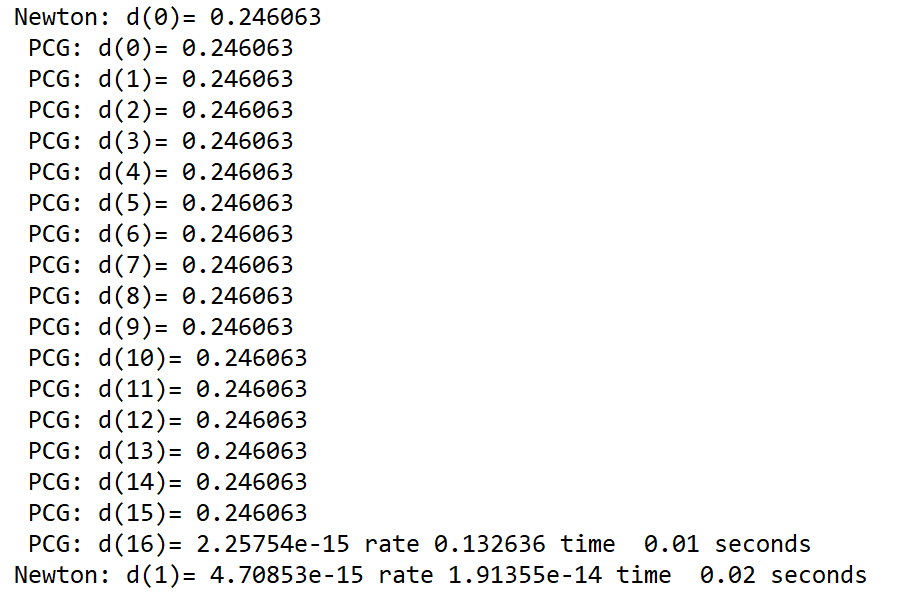
\includegraphics[width=0.5\textwidth]{../../Aufgabe10/blubblub.png}}	 
\end{figure}

Wir erhalten so für die Level $3, \dots,9$ die folgenden Werte:

\begin{figure}[H]
	\centering
	\captionabove{Iterativer Löser: CG-Verfahren, Vorkonditionierer: Jacobi}
	\subfigure{\includegraphics[width=0.67\textwidth]{../../Aufgabe10/Jacobi-CG.png}}	 
\end{figure}

Man sieht dabei außerdem sehr schön, dass für jedes Level stets doppelt so viele Iterationschritte benötigt werden, wie im vorherigen. Außerdem sieht man, dass die Konvergenzrate wie zu erwarten bei höherem Level schlechter wird. 
%Für GMRES und CG kenne wir folgende Fehlerabschätzungen:
%\begin{align*}
%&Ax = b \text{ mit Vorkonditionierern } B\\
%&\text{GMRES: }&&&& \text{CG: }\\
%&\abs{x^k-x}_2 \le \kappa_2(BA) \sqrt{1 - \frac{\alpha^2}{C^2}} \abs{x^0 - x}_2 &&&& \abs{x^k - x}_A \le 2 \left( \frac{\sqrt{\kappa_2(BA)} - 1}{\sqrt{\kappa_2(BA)} + 1} \right)^k \abs{x^0 - x}_A
%\end{align*}
Durch die Fehlerschranken für GMRES und CG motiviert, liegt es nahe, dass die Größen aus der Tabelle folgendermaßen zusammen hängen:

\[\text{Fehler 2}= \text{Rate}^{\text{Iterationsschritt}} \cdot \text{Fehler 1}\]

Somit ist eine \enquote{Rate} nahe bei 0 gut, eine \enquote{Rate} nahe bei 1 schlecht im Bezug auf Eignung des verwendeten Verfahrens. 

Anschließend können wir die Ergebnisse auch noch mit der Anwendung des Jacobi-Vorkonditionierers auf das GMRES-Verfahren zum gleichen Problem vergleichen:

\begin{figure}[H]
	\centering
	\captionabove{Iterativer Löser: GMRES-Verfahren, Vorkonditionierer: Jacobi}
	\subfigure{\includegraphics[width=0.33\textwidth]{../../Aufgabe10/Jacobi-GMRES.png}}	 
\end{figure}

Hierbei fällt sehr schnell die extreme Verschlechterung der Konvergenzrate zwischen den Leveln 6 und 7.
Bis Level 6 verhalten sich die so entstehenden Ergebnisse noch sehr ähnlich, wie zuvor beim CG-Verfahren.
Ab Level 7 hingegen ist die Konvergenzrate sehr schlecht (nahe 1) und der iterative Löser bricht erst nach 800 (das ist bereits die eingestellte maximale Schrittanzahl des iterativen Lösers) ab. 
%Dies lässt sich auf folgenden Sachverhalt zurückführen:
%\textcolor{red}{WOHER ZUM TEUFEL SOLL ICH DAS WISSEN HINWEIS REDUZIERUNG DES SPEICHERBEDARFS}
\newline
Anschließend haben wir die bereits beschriebenen Ergebnisse mit denen von weiteren Vorkonditionierer/Löser-Kombinationen verglichen:

\begin{figure}[H]
	\centering
	\captionabove{Weitere Iterative Löser mit verschiedenen Vorkonditionierern}
	\subfigure{\includegraphics[width=0.99\textwidth]{../../Aufgabe10/blub.png}}	 
\end{figure}

Besonders fallen hier die Verfahren mit Multigrid-Konditionierer auf, welche beide sehr gute Konvergenzraten bei sehr wenigen Iterationsschritten vorweisen.
Weiter sieht man, dass das symmetrische GaussSeidel-Verfahren sich noch zumindest annehmbar gut als Vorkonditionierer für das CG-Verfahren eignet, während ein GaussSeidel-Vorkonditionierer kombiniert mit dem GMRES-Verfahren ähnlich schlecht abschneidet, wie zuvor das GMRES-Verfahren mit Jacobi-Vorkonditionierer.
Grundsätzlich sieht man, dass es  sich lohnen kann, für ein symmetrisches Problem wie Simple2D das CG-Verfahren zu nutzen.
\newline
In der in Aufgabe 11 gestellten Bonusaufgabe haben wir uns dann noch mit den folgenden drei Fragen beschäftigt: Wie ändert sich das Verhalten, wenn 
\begin{enumerate}
	\item das Programm auf mehreren Prozessoren gestartet wird:
	\begin{figure}[H]
		\centering
		\captionabove{Jacobi-CG auf Lvl 9 mit 1,2 und 4 Prozessoren}
		\subfigure[1 Prozessor]{\includegraphics[width=0.77\textwidth]{../../Aufgabe10/proc1lvl9.png}}	 
		\subfigure[2 Prozessoren]{\includegraphics[width=0.77\textwidth]{../../Aufgabe10/proc2lvl9.png}}	 
		\subfigure[4 Prozessoren]{\includegraphics[width=0.77\textwidth]{../../Aufgabe10/proc4lvl9.png}}	 
	\end{figure}
    
    Trotz unterschiedlicher Anzahl an Prozessoren wird, wie man an obigem Vergleich leicht einsieht, stets dieselbe Anzahl an Iterationsschritten für den linearen Löser benötigt.
    

	\item das Programm für andere Probleme (Discontinuous, Divergent) verwendet wird:
	\begin{figure}[H]
		\centering
		\captionabove{Jacobi-GMRES auf Lvl 6 für verschiedene Probleme}
	\subfigure[Problem Simple 2D]{\includegraphics[width=0.77\textwidth]{../../Aufgabe10/simple.png}}	 
	\subfigure[Problem Discontinuous]{\includegraphics[width=0.77\textwidth]{../../Aufgabe10/disco.png}}	 
	\subfigure[Problem Divergent]{\includegraphics[width=0.77\textwidth]{../../Aufgabe10/divergent.png}}	 
		\end{figure}
	Man sieht, dass die Anzahl der benötigten Iterationsschritte stark vom zugrunde liegenden Problem abhängt. 
	
    
	
	\item wir anstatt eines Krylow-UVR-Verfahrens einen linearen Löser ohne Dämpfung verwenden.
	
	\begin{figure}[H]
		\centering
		\captionabove{Jacobi-CG auf Lvl 9 mit 1,2 und 4 Prozessoren}
		\subfigure[Jacobi-CG Verfahren]{\includegraphics[width=0.77\textwidth]{../../Aufgabe10/CG3.png}}	 
		\subfigure[Linearer Löser ohne Dämpfung]{\includegraphics[width=0.77\textwidth]{../../Aufgabe10/LS3.png}}	 
		
	\end{figure}
	
	Ein linearer Löser ohne Dämpfung ist im Gegensatz zu den vorgestellten Krylow-UVR-Verfahren relativ schlecht für die Lösung des Problems geeignet. 
\end{enumerate}



\end{document}

